In ATLAS analyses structured similarly to those in this dissertation, Monte Carlo statistics can often play a substantial part in driving systematic uncertainty. If the templates used to perform the spurious signal study contain a large number of statistical fluctuations, the spurious signal will often be an overestimate due to the tendency to fit statistical fluctuations in the templates as legitimate spurious signal. Though producing more Monte Caro simulated samples would resolve this issue, it is often computationally intensive and inefficient.

In order to resolve this, a technique known as Gaussian Process Regression is implemented in the context of the Couplings analysis. This is implemented using the Gaussian Smoothing for BackGrounds (GaSBaG) tool first developed in \cite{Hyneman}, which interfaces with the Scikit-Learn \cite{scikit-learn} machine learning package.

A Gaussian Process (GP) is defined as a set of random processes of which all finite subsets have a multivariate normal distribution \cite{ebden2015gaussian}. Provided statistics in each bin are high enough, a histogram encoding some underlying smooth distribution is an example of such a finite subset: each bin contains a normally-distributed number of events about some true mean, and the bins are correlated according to their covariance. Thus, a Gaussian process can be defined over such a histogram. The mean of the fitted Gaussian Process corresponds to the smooth underlying shape, while the elements of the GP covariance matrix correspond to the error in each bin and the correlation between bins.

The covariance matrix can be simplified using a kernel, which determines the form of the correlation between points. Useful kernel functions parameterize the dependence between two such points in terms of one or more "length scale" hyparameters, which determine the distance in X at which two points are expected to influence one another in Y. Two such kernels are the constant-length-scale Radial Basis Function (RBF) kernel \cite{3569} and the variable-length-scale Gibbs kernel \cite{Gibbs}. 

The RBF kernel has one hyperparameter, the constant length scale $l$, and it is defined as

\begin{equation}
K_\text{RBF}(x,x') = exp\left(\frac{-(x-x')^2}{2l^2}\right)
\end{equation}

The RBF kernel performs optimally on linear functions. However, for smoothly-falling functions that are not necessarily linear, it is likely that nearby points will be more correlated in some regimes than in others, so a constant length scale is likely a suboptimal model for nonlinear functions. The Gibbs kernel allows the length scale to vary linearly as a function of $x$, that is, ${l(x)=l_{0}+l_{1}(x)}$. It has two hyperparameters: the initial length scale $l_{0}$ and the length scale slope $l_{1}$. The Gibbs kernel function is: 

\begin{equation}
K_\text{Gibbs}(x, x') = \frac{\sqrt{2l(x)l(x')}}{l(x)^2 + l(x')^2 } \cdot exp\left( \frac{-(x-x')^2}{l(x)^2 + l(x')^2} \right)
\end{equation}


It is assumed that the "true" underlying functional form of the background in each category is a smoothly falling function; the background templates used in the Couplings analysis are all smoothly falling distributions with statistical fluctuations. By utilizing a Gaussian Process Regression fit and then taking the mean of the Gaussian Process as the "true" template shape, it is possible to reduce the statistical noise, thus decreasing the spurious signal systematic. The GP smoothing technique assumes nothing about the form of the underlying distribution other than that it is smooth and falling, so the smoothing procedure should not bias the spurious signal test toward a particular functional shape.

The hyperparameters (initial length scale and length scale slope) are allowed to vary over a user-specified range; the optimal hyperparameters within this range are then determined as part of the Gaussian Process fit.

A GP is fit to the background template in each category. This can be modelled in a Bayesian manner: the GP is a distribution with a given prior mean that is then conditioned on the template histogram; the smoothed template is the mean of the posterior distribution \cite{3569}. Due to the expected shape of the templates, the prior is defined as an exponential function with parameters obtained by a fit to the template. However, in cases where the input template has very few statistics, large errors on the data points are compatible with a steep exponential prior though the "true" underlying shape is approximately flat, which can confound the fitter and cause it to simply output the prior distribution. Therefore, a "switch" has been added to re-perform the GP fit using a flat prior in cases where the resulting GP shape and the prior exponential shape disagree with a $\chi^2/DoF < 0.1$.

The mean of the GP posterior is then saved as the new template (with bin-by-bin errors corresponding to the bin-by-bin errors of the original template). The spurious signal test is then performed with these new distributions.

Validation tests were performed with the GP smoothing technique in order to quantify whether or not GPR induces a bias (that is, artifically reduces the spurious signal beyond just smoothing out statistical fluctuations). These tests primarily use “toy” templates- randomly-generated background templates constructed using a known analytic function as a probability density. One of the goals of these validation studies is to determine a safe statistical regime in which to apply GPR, as in the very low-statistics regime, the distribution of events in each bin follows a Poisson distribution rather than a Gaussian distribution.

We find that GPR remains effectively unbiased for smoothly-falling templates containing more than an average of 20 Monte Carlo events/ bin. The procedures to validate the GPR smoothing are reported in Appendix \ref{app:gpr_validation}.

\section{Gaussian Processes smoothed background templates}
\label{sec:GPR_templates}

The background templates of all of the Coupling analysis categories, both before and after the Gaussian Processes (GP) smoothing, are presented in \Figrange{\ref{fig:gpr_coupcat_1}}{\ref{fig:gpr_coupcat_22}}. The data sidebands, corresponding to \SI{139}{\per\fb}, are shown for comparison, although the GP smoothing technique does not take them into account.

As detailed in \ref{sec:GPR_validation}, the GPR method chosen for use in the Couplings analysis involves extending our templates by 5 GeV on either side to reduce edge effects, as well as the choice of a linear error kernel in order to properly handle template errors.

\begin{figure} 
\begin{center}
\begin{subfigure}[T]{0.49\linewidth}
	\centering
	\includegraphics[width=\linewidth]{figures/background/gpr/coupCatTemplates/GPR_Smoothed_Plot_hmgg_c0.eps}
	\caption{GG2H\_0J\_PTH\_0\_10\_\_0}
\end{subfigure}
\begin{subfigure}[T]{0.49\linewidth}
	\centering
	\includegraphics[width=\linewidth]{figures/background/gpr/coupCatTemplates/GPR_Smoothed_Plot_hmgg_c1.eps}
	\caption{GG2H\_0J\_PTH\_GT10\_\_0}
\end{subfigure}
\begin{subfigure}[T]{0.49\linewidth}
	\centering
	\includegraphics[width=\linewidth]{figures/background/gpr/coupCatTemplates/GPR_Smoothed_Plot_hmgg_2Merge4_c0.eps}
	\caption{GG2H\_1J\_PTH\_0\_60}
\end{subfigure}
\begin{subfigure}[T]{0.49\linewidth}
	\centering
	\includegraphics[width=\linewidth]{figures/background/gpr/coupCatTemplates/GPR_Smoothed_Plot_hmgg_2Merge4_c1.eps}
	\caption{GG2H\_1J\_PTH\_60\_120}
\end{subfigure}
\caption{The full Run 2 background templates of the labelled categories. The red shape shows the original background template, the blue shape shows the smoothed background template, and the black points show the data sidebands (for reference). The bottom panel shows the fractional difference between the smoothed and un-smoothed templates and the data sidebands.}
\label{fig:gpr_coupcat_1}
\end{center}
\end{figure}


\begin{figure} 
\begin{center}
\begin{subfigure}[T]{0.49\linewidth}
	\centering
	\includegraphics[width=\linewidth]{figures/background/gpr/coupCatTemplates/GPR_Smoothed_Plot_hmgg_c6.eps}
	\caption{GG2H\_1J\_PTH\_120\_200\_\_0}
\end{subfigure}
\begin{subfigure}[T]{0.49\linewidth}
	\centering
	\includegraphics[width=\linewidth]{figures/background/gpr/coupCatTemplates/GPR_Smoothed_Plot_hmgg_c7.eps}
	\caption{GG2H\_1J\_PTH\_120\_200\_\_1}
\end{subfigure}
\begin{subfigure}[T]{0.49\linewidth}
	\centering
	\includegraphics[width=\linewidth]{figures/background/gpr/coupCatTemplates/GPR_Smoothed_Plot_hmgg_c8.eps}
	\caption{GG2H\_GE2J\_MJJ\_0\_350\_PTH\_0\_60\_\_0}
\end{subfigure}
\begin{subfigure}[T]{0.49\linewidth}
	\centering
	\includegraphics[width=\linewidth]{figures/background/gpr/coupCatTemplates/GPR_Smoothed_Plot_hmgg_c9.eps}
	\caption{GG2H\_GE2J\_MJJ\_0\_350\_PTH\_0\_60\_\_1}
\end{subfigure}
\caption{The Couplings-Analysis background templates in the indicated categories. The red histogram is the unsmoothed background template, the blue histogram is the smoothed background template, and the black points show the data sidebands. The bottom panel shows the per-bin percent deviation of both the smoothed and unsmoothed templates from the data sidebands. }
\label{fig:gpr_coupcat_2}
\end{center}
\end{figure}

\begin{figure} 
\begin{center}
\begin{subfigure}[T]{0.49\linewidth}
	\centering
	\includegraphics[width=\linewidth]{figures/background/gpr/coupCatTemplates/GPR_Smoothed_Plot_hmgg_c10.eps}
	\caption{GG2H\_GE2J\_MJJ\_0\_350\_PTH\_0\_60\_\_2}
\end{subfigure}
\begin{subfigure}[T]{0.49\linewidth}
	\centering
	\includegraphics[width=\linewidth]{figures/background/gpr/coupCatTemplates/GPR_Smoothed_Plot_hmgg_c11.eps}
	\caption{GG2H\_GE2J\_MJJ\_0\_350\_PTH\_60\_120\_\_0}
\end{subfigure}
\begin{subfigure}[T]{0.49\linewidth}
	\centering
	\includegraphics[width=\linewidth]{figures/background/gpr/coupCatTemplates/GPR_Smoothed_Plot_hmgg_c12.eps}
	\caption{GG2H\_GE2J\_MJJ\_0\_350\_PTH\_60\_120\_\_1}
\end{subfigure}
\begin{subfigure}[T]{0.49\linewidth}
	\centering
	\includegraphics[width=\linewidth]{figures/background/gpr/coupCatTemplates/GPR_Smoothed_Plot_hmgg_c13.eps}
	\caption{GG2H\_GE2J\_MJJ\_0\_350\_PTH\_60\_120\_\_2}
\end{subfigure}
\caption{The Couplings-Analysis background templates in the indicated categories. The red histogram is the unsmoothed background template, the blue histogram is the smoothed background template, and the black points show the data sidebands. The bottom panel shows the per-bin percent deviation of both the smoothed and unsmoothed templates from the data sidebands. }
\label{fig:gpr_coupcat_3}
\end{center}
\end{figure}

\begin{figure}
\begin{center}
\begin{subfigure}[T]{0.49\linewidth}
	\centering
	\includegraphics[width=\linewidth]{figures/background/gpr/coupCatTemplates/GPR_Smoothed_Plot_hmgg_c14.eps}
	\caption{\tiny{GG2H\_GE2J\_MJJ\_0\_350\_PTH\_120\_200\_\_0}}
\end{subfigure}
\begin{subfigure}[T]{0.49\linewidth}
	\centering
	\includegraphics[width=\linewidth]{figures/background/gpr/coupCatTemplates/GPR_Smoothed_Plot_hmgg_c15.eps}
	\caption{\tiny{GG2H\_GE2J\_MJJ\_0\_350\_PTH\_120\_200\_\_1}}
\end{subfigure}
\begin{subfigure}[T]{0.49\linewidth}
	\centering
	\includegraphics[width=\linewidth]{figures/background/gpr/coupCatTemplates/GPR_Smoothed_Plot_hmgg_c16.eps}
	\caption{\tiny{GG2H\_GE2J\_MJJ\_350\_700\_PTH\_0\_200\_PTHJJ\_0\_25\_\_0}}
\end{subfigure}
\begin{subfigure}[T]{0.49\linewidth}
	\centering
	\includegraphics[width=\linewidth]{figures/background/gpr/coupCatTemplates/GPR_Smoothed_Plot_hmgg_c17.eps}
	\caption{\tiny{GG2H\_GE2J\_MJJ\_350\_700\_PTH\_0\_200\_PTHJJ\_0\_25\_\_1}}
\end{subfigure}
\caption{The Couplings-Analysis background templates in the indicated categories. The red histogram is the unsmoothed background template, the blue histogram is the smoothed background template, and the black points show the data sidebands. The bottom panel shows the per-bin percent deviation of both the smoothed and unsmoothed templates from the data sidebands. }
 \label{fig:gpr_coupcat_4}
 \end{center}
\end{figure}

\begin{figure}
\begin{center}
\begin{subfigure}[T]{0.49\linewidth}
	\centering
	\includegraphics[width=\linewidth]{figures/background/gpr/coupCatTemplates/GPR_Smoothed_Plot_hmgg_c18.eps}
	\caption{\tiny{GG2H\_GE2J\_MJJ\_350\_700\_PTH\_0\_200\_PTHJJ\_0\_25\_\_2}}
\end{subfigure}
\begin{subfigure}[T]{0.49\linewidth}
	\centering
	\includegraphics[width=\linewidth]{figures/background/gpr/coupCatTemplates/GPR_Smoothed_Plot_hmgg_c19.eps}
	\caption{\tiny{GG2H\_GE2J\_MJJ\_350\_700\_PTH\_0\_200\_PTHJJ\_GT25\_\_0}}
\end{subfigure}
\begin{subfigure}[T]{0.49\linewidth}
	\centering
	\includegraphics[width=\linewidth]{figures/background/gpr/coupCatTemplates/GPR_Smoothed_Plot_hmgg_c20.eps}
	\caption{\tiny{GG2H\_GE2J\_MJJ\_350\_700\_PTH\_0\_200\_PTHJJ\_GT25\_\_1}}
\end{subfigure}
\begin{subfigure}[T]{0.49\linewidth}
	\centering
	\includegraphics[width=\linewidth]{figures/background/gpr/coupCatTemplates/GPR_Smoothed_Plot_hmgg_c21.eps}
	\caption{\tiny{GG2H\_GE2J\_MJJ\_350\_700\_PTH\_0\_200\_PTHJJ\_GT25\_\_2}}
\end{subfigure}
\caption{The Couplings-Analysis background templates in the indicated categories. The red histogram is the unsmoothed background template, the blue histogram is the smoothed background template, and the black points show the data sidebands. The bottom panel shows the per-bin percent deviation of both the smoothed and unsmoothed templates from the data sidebands. }
 \label{fig:gpr_coupcat_5}
 \end{center}
\end{figure}

\begin{figure} 
\begin{center}
\begin{subfigure}[T]{0.49\linewidth}
	\centering
	\includegraphics[width=\linewidth]{figures/background/gpr/coupCatTemplates/GPR_Smoothed_Plot_hmgg_c22.eps}
	\caption{\tiny{GG2H\_GE2J\_MJJ\_GT700\_PTH\_0\_200\_PTHJJ\_0\_25\_\_0}}
\end{subfigure}
\begin{subfigure}[T]{0.49\linewidth}
	\centering
	\includegraphics[width=\linewidth]{figures/background/gpr/coupCatTemplates/GPR_Smoothed_Plot_hmgg_c23.eps}
	\caption{\tiny{GG2H\_GE2J\_MJJ\_GT700\_PTH\_0\_200\_PTHJJ\_0\_25\_\_1}}
\end{subfigure}
\begin{subfigure}[T]{0.49\linewidth}
	\centering
	\includegraphics[width=\linewidth]{figures/background/gpr/coupCatTemplates/GPR_Smoothed_Plot_hmgg_c24.eps}
	\caption{\tiny{GG2H\_GE2J\_MJJ\_GT700\_PTH\_0\_200\_PTHJJ\_0\_25\_\_2}}
\end{subfigure}
\begin{subfigure}[T]{0.49\linewidth}
	\centering
	\includegraphics[width=\linewidth]{figures/background/gpr/coupCatTemplates/GPR_Smoothed_Plot_hmgg_c25.eps}
	\caption{\tiny{GG2H\_GE2J\_MJJ\_GT700\_PTH\_0\_200\_PTHJJ\_GT25\_\_0}}
\end{subfigure}
\caption{The Couplings-Analysis background templates in the indicated categories. The red histogram is the unsmoothed background template, the blue histogram is the smoothed background template, and the black points show the data sidebands. The bottom panel shows the per-bin percent deviation of both the smoothed and unsmoothed templates from the data sidebands. }
\label{fig:gpr_coupcat_6}
\end{center}
\end{figure}

\begin{figure}
\begin{center}
\begin{subfigure}[T]{0.49\linewidth}
	\centering
	\includegraphics[width=\linewidth]{figures/background/gpr/coupCatTemplates/GPR_Smoothed_Plot_hmgg_c26.eps}
	\caption{\tiny{GG2H\_GE2J\_MJJ\_GT700\_PTH\_0\_200\_PTHJJ\_GT25\_\_1}}
\end{subfigure}
\begin{subfigure}[T]{0.49\linewidth}
	\centering
	\includegraphics[width=\linewidth]{figures/background/gpr/coupCatTemplates/GPR_Smoothed_Plot_hmgg_c27.eps}
	\caption{\tiny{GG2H\_GE2J\_MJJ\_GT700\_PTH\_0\_200\_PTHJJ\_GT25\_\_2}}
\end{subfigure}
\begin{subfigure}[T]{0.49\linewidth}
	\centering
	\includegraphics[width=\linewidth]{figures/background/gpr/coupCatTemplates/GPR_Smoothed_Plot_hmgg_c28.eps}
	\caption{GG2H\_PTH\_200\_300\_\_0}
\end{subfigure}
\begin{subfigure}[T]{0.49\linewidth}
	\centering
	\includegraphics[width=\linewidth]{figures/background/gpr/coupCatTemplates/GPR_Smoothed_Plot_hmgg_c29.eps}
	\caption{GG2H\_PTH\_200\_300\_\_1}
\end{subfigure}
	\caption{The Couplings-Analysis background templates in the indicated categories. The red histogram is the unsmoothed background template, the blue histogram is the smoothed background template, and the black points show the data sidebands. The bottom panel shows the per-bin percent deviation of both the smoothed and unsmoothed templates from the data sidebands. }
 \label{fig:gpr_coupcat_7}
 \end{center}
\end{figure}

\begin{figure}
\begin{center}
\begin{subfigure}[T]{0.49\linewidth}
	\centering
	\includegraphics[width=\linewidth]{figures/background/gpr/coupCatTemplates/GPR_Smoothed_Plot_hmgg_c30.eps}
	\caption{GG2H\_PTH\_200\_300\_\_2}
\end{subfigure}
%\begin{subfigure}[T]{0.49\linewidth}
%	\centering
%	\includegraphics[width=\linewidth]{figures/background/gpr/coupCatTemplates/GPR_Smoothed_Plot_hmgg_c31.eps}
%	\caption{GG2H\_PTH\_300\_450\_\_0}
%\end{subfigure}
\begin{subfigure}[T]{0.49\linewidth}
	\centering
	\includegraphics[width=\linewidth]{figures/background/gpr/coupCatTemplates/GPR_Smoothed_Plot_hmgg_c32.eps}
	\caption{GG2H\_PTH\_300\_450\_\_1}
\end{subfigure}
\begin{subfigure}[T]{0.49\linewidth}
	\centering
	\includegraphics[width=\linewidth]{figures/background/gpr/coupCatTemplates/GPR_Smoothed_Plot_hmgg_c33.eps}
	\caption{GG2H\_PTH\_300\_450\_\_2}
\end{subfigure}
	\caption{The Couplings-Analysis background templates in the indicated categories. The red histogram is the unsmoothed background template, the blue histogram is the smoothed background template, and the black points show the data sidebands. The bottom panel shows the per-bin percent deviation of both the smoothed and unsmoothed templates from the data sidebands. }
 \label{fig:gpr_coupcat_8}
 \end{center}
\end{figure}

\begin{figure}
\begin{center}
%\begin{subfigure}[T]{0.49\linewidth}
%	\centering
%	\includegraphics[width=\linewidth]{figures/background/gpr/coupCatTemplates/GPR_Smoothed_Plot_hmgg_c34.eps}
%	\caption{GG2H\_PTH\_450\_650\_\_0}
%\end{subfigure}
\begin{subfigure}[T]{0.49\linewidth}
	\centering
	\includegraphics[width=\linewidth]{figures/background/gpr/coupCatTemplates/GPR_Smoothed_Plot_hmgg_c35New.eps}
	\caption{GG2H\_PTH\_450\_650\_\_1}
\end{subfigure}
%\begin{subfigure}[T]{0.49\linewidth}
%	\centering
%	\includegraphics[width=\linewidth]{figures/background/gpr/coupCatTemplates/GPR_Smoothed_Plot_hmgg_c36.eps}
%	\caption{GG2H\_PTH\_GT650\_\_0}
%\end{subfigure}
%\begin{subfigure}[T]{0.49\linewidth}
%	\centering
%	\includegraphics[width=\linewidth]{figures/background/gpr/coupCatTemplates/GPR_Smoothed_Plot_hmgg_c37.eps}
%	\caption{GG2H\_PTH\_GT650\_\_1}
%\end{subfigure}
\caption{The Couplings-Analysis background templates in the indicated categories. The red histogram is the unsmoothed background template, the blue histogram is the smoothed background template, and the black points show the data sidebands. The bottom panel shows the per-bin percent deviation of both the smoothed and unsmoothed templates from the data sidebands. }
 \label{fig:gpr_coupcat_9}
 \end{center}
\end{figure}

\begin{figure}
\begin{center}
%\begin{subfigure}[T]{0.49\linewidth}
%	\centering
%	\includegraphics[width=\linewidth]{figures/background/gpr/coupCatTemplates/GPR_Smoothed_Plot_hmgg_c38.eps}
%	\caption{QQ2HQQ\_0J\_\_0}
%\end{subfigure}
\begin{subfigure}[T]{0.49\linewidth}
	\centering
	\includegraphics[width=\linewidth]{figures/background/gpr/coupCatTemplates/GPR_Smoothed_Plot_hmgg_c39.eps}
	\caption{QQ2HQQ\_0J\_\_1}
\end{subfigure}
%\begin{subfigure}[T]{0.49\linewidth}
%	\centering
%	\includegraphics[width=\linewidth]{figures/background/gpr/coupCatTemplates/GPR_Smoothed_Plot_hmgg_c40.eps}
%	\caption{QQ2HQQ\_1J\_\_0}
%\end{subfigure}
\begin{subfigure}[T]{0.49\linewidth}
	\centering
	\includegraphics[width=\linewidth]{figures/background/gpr/coupCatTemplates/GPR_Smoothed_Plot_hmgg_c41.eps}
	\caption{QQ2HQQ\_1J\_\_1}
\end{subfigure}
\caption{The Couplings-Analysis background templates in the indicated categories. The red histogram is the unsmoothed background template, the blue histogram is the smoothed background template, and the black points show the data sidebands. The bottom panel shows the per-bin percent deviation of both the smoothed and unsmoothed templates from the data sidebands. }
 \label{fig:gpr_coupcat_10}
 \end{center}
\end{figure}

\begin{figure} 
\begin{center}
\begin{subfigure}[T]{0.49\linewidth}
	\centering
	\includegraphics[width=\linewidth]{figures/background/gpr/coupCatTemplates/GPR_Smoothed_Plot_hmgg_c42.eps}
	\caption{QQ2HQQ\_1J\_\_2}
\end{subfigure}
%\begin{subfigure}[T]{0.49\linewidth}
%	\centering
%	\includegraphics[width=\linewidth]{figures/background/gpr/coupCatTemplates/GPR_Smoothed_Plot_hmgg_c43.eps}
%	\caption{QQ2HQQ\_GE2J\_MJJ\_0\_60\_\_0}
%\end{subfigure}
\begin{subfigure}[T]{0.49\linewidth}
	\centering
	\includegraphics[width=\linewidth]{figures/background/gpr/coupCatTemplates/GPR_Smoothed_Plot_hmgg_c44.eps}
	\caption{QQ2HQQ\_GE2J\_MJJ\_0\_60\_\_1}
\end{subfigure}
\begin{subfigure}[T]{0.49\linewidth}
	\centering
	\includegraphics[width=\linewidth]{figures/background/gpr/coupCatTemplates/GPR_Smoothed_Plot_hmgg_c45.eps}
	\caption{QQ2HQQ\_GE2J\_MJJ\_0\_60\_\_2}
\end{subfigure}
\caption{The Couplings-Analysis background templates in the indicated categories. The red histogram is the unsmoothed background template, the blue histogram is the smoothed background template, and the black points show the data sidebands. The bottom panel shows the per-bin percent deviation of both the smoothed and unsmoothed templates from the data sidebands. }
\label{fig:gpr_coupcat_11}
\end{center}
\end{figure}

\begin{figure}
\begin{center}
\begin{subfigure}[T]{0.49\linewidth}
	\centering
	\includegraphics[width=\linewidth]{figures/background/gpr/coupCatTemplates/GPR_Smoothed_Plot_hmgg_c46.eps}
	\caption{QQ2HQQ\_GE2J\_MJJ\_60\_120\_\_0}
\end{subfigure}
\begin{subfigure}[T]{0.49\linewidth}
	\centering
	\includegraphics[width=\linewidth]{figures/background/gpr/coupCatTemplates/GPR_Smoothed_Plot_hmgg_c47.eps}
	\caption{QQ2HQQ\_GE2J\_MJJ\_60\_120\_\_1}
\end{subfigure}
%\begin{subfigure}[T]{0.49\linewidth}
%	\centering
%	\includegraphics[width=\linewidth]{figures/background/gpr/coupCatTemplates/GPR_Smoothed_Plot_hmgg_c48.eps}
%	\caption{QQ2HQQ\_GE2J\_MJJ\_120\_350\_\_0}
%\end{subfigure}
\begin{subfigure}[T]{0.49\linewidth}
	\centering
	\includegraphics[width=\linewidth]{figures/background/gpr/coupCatTemplates/GPR_Smoothed_Plot_hmgg_c49.eps}
	\caption{QQ2HQQ\_GE2J\_MJJ\_120\_350\_\_1}
\end{subfigure}
\caption{The Couplings-Analysis background templates in the indicated categories. The red histogram is the unsmoothed background template, the blue histogram is the smoothed background template, and the black points show the data sidebands. The bottom panel shows the per-bin percent deviation of both the smoothed and unsmoothed templates from the data sidebands. }
 \label{fig:gpr_coupcat_12}
 \end{center}
\end{figure}

\begin{figure}
\begin{center}
\begin{subfigure}[T]{0.49\linewidth}
	\centering
	\includegraphics[width=\linewidth]{figures/background/gpr/coupCatTemplates/GPR_Smoothed_Plot_hmgg_c50.eps}
	\caption{\tiny{QQ2HQQ\_GE2J\_MJJ\_120\_350\_\_2}}
\end{subfigure}
%\begin{subfigure}[T]{0.49\linewidth}
%	\centering
%	\includegraphics[width=\linewidth]{figures/background/gpr/coupCatTemplates/GPR_Smoothed_Plot_hmgg_c51.eps}
%	\caption{\tiny{QQ2HQQ\_GE2J\_MJJ\_350\_700\_PTH\_0\_200\_PTHJJ\_0\_25\_\_0}}
%\end{subfigure}
\begin{subfigure}[T]{0.49\linewidth}
	\centering
	\includegraphics[width=\linewidth]{figures/background/gpr/coupCatTemplates/GPR_Smoothed_Plot_hmgg_c52.eps}
	\caption{\tiny{QQ2HQQ\_GE2J\_MJJ\_350\_700\_PTH\_0\_200\_PTHJJ\_0\_25\_\_1}}
\end{subfigure}
%\begin{subfigure}[T]{0.49\linewidth}
%	\centering
%	\includegraphics[width=\linewidth]{figures/background/gpr/coupCatTemplates/GPR_Smoothed_Plot_hmgg_c53.eps}
%	\caption{\tiny{QQ2HQQ\_GE2J\_MJJ\_350\_700\_PTH\_0\_200\_PTHJJ\_GT25\_\_0}}
%\end{subfigure}
\caption{The Couplings-Analysis background templates in the indicated categories. The red histogram is the unsmoothed background template, the blue histogram is the smoothed background template, and the black points show the data sidebands. The bottom panel shows the per-bin percent deviation of both the smoothed and unsmoothed templates from the data sidebands. }
 \label{fig:gpr_coupcat_13}
 \end{center}
\end{figure}

\begin{figure}
\begin{center}
%\begin{subfigure}[T]{0.49\linewidth}
%	\centering
%	\includegraphics[width=\linewidth]{figures/background/gpr/coupCatTemplates/GPR_Smoothed_Plot_hmgg_c54.eps}
%	\caption{\tiny{QQ2HQQ\_GE2J\_MJJ\_350\_700\_PTH\_0\_200\_PTHJJ\_GT25\_\_1}}
%\end{subfigure}
%\begin{subfigure}[T]{0.49\linewidth}
%	\centering
%	\includegraphics[width=\linewidth]{figures/background/gpr/coupCatTemplates/GPR_Smoothed_Plot_hmgg_c55.eps}
%	\caption{\tiny{QQ2HQQ\_GE2J\_MJJ\_GT700\_PTH\_0\_200\_PTHJJ\_0\_25\_\_0}}
%\end{subfigure}
\begin{subfigure}[T]{0.49\linewidth}
	\centering
	\includegraphics[width=\linewidth]{figures/background/gpr/coupCatTemplates/GPR_Smoothed_Plot_hmgg_c56.eps}
	\caption{\tiny{QQ2HQQ\_GE2J\_MJJ\_GT700\_PTH\_0\_200\_PTHJJ\_0\_25\_\_1}}
\end{subfigure}
%\begin{subfigure}[T]{0.49\linewidth}
%	\centering
%	\includegraphics[width=\linewidth]{figures/background/gpr/coupCatTemplates/GPR_Smoothed_Plot_hmgg_c57.eps}
%	\caption{\tiny{QQ2HQQ\_GE2J\_MJJ\_GT700\_PTH\_0\_200\_PTHJJ\_GT25\_\_0}}
%\end{subfigure}
\caption{The Couplings-Analysis background templates in the indicated categories. The red histogram is the unsmoothed background template, the blue histogram is the smoothed background template, and the black points show the data sidebands. The bottom panel shows the per-bin percent deviation of both the smoothed and unsmoothed templates from the data sidebands. }
 \label{fig:gpr_coupcat_14}
 \end{center}
\end{figure}

\begin{figure}
\begin{center}
%\begin{subfigure}[T]{0.49\linewidth}
%	\centering
%	\includegraphics[width=\linewidth]{figures/background/gpr/coupCatTemplates/GPR_Smoothed_Plot_hmgg_c58.eps}
%	\caption{\tiny{QQ2HQQ\_GE2J\_MJJ\_GT700\_PTH\_0\_200\_PTHJJ\_GT25\_\_1}}
%\end{subfigure}
\begin{subfigure}[T]{0.49\linewidth}
	\centering
	\includegraphics[width=\linewidth]{figures/background/gpr/coupCatTemplates/GPR_Smoothed_Plot_hmgg_c59.eps}
	\caption{\tiny{QQ2HQQ\_GE2J\_MJJ\_GT700\_PTH\_0\_200\_PTHJJ\_GT25\_\_2}}
\end{subfigure}
%\begin{subfigure}[T]{0.49\linewidth}
%	\centering
%	\includegraphics[width=\linewidth]{figures/background/gpr/coupCatTemplates/GPR_Smoothed_Plot_hmgg_c60.eps}
%	\caption{\tiny{QQ2HQQ\_GE2J\_MJJ\_350\_700\_PTH\_GT200\_\_0}}
%\end{subfigure}
%\begin{subfigure}[T]{0.49\linewidth}
%	\centering
%	\includegraphics[width=\linewidth]{figures/background/gpr/coupCatTemplates/GPR_Smoothed_Plot_hmgg_c61.eps}
%	\caption{\tiny{QQ2HQQ\_GE2J\_MJJ\_350\_700\_PTH\_GT200\_\_1}}
%\end{subfigure}
\caption{The Couplings-Analysis background templates in the indicated categories. The red histogram is the unsmoothed background template, the blue histogram is the smoothed background template, and the black points show the data sidebands. The bottom panel shows the per-bin percent deviation of both the smoothed and unsmoothed templates from the data sidebands. }
 \label{fig:gpr_coupcat_15}
 \end{center}
\end{figure}

\begin{figure} 
\begin{center}
%\begin{subfigure}[T]{0.49\linewidth}
%	\centering
%	\includegraphics[width=\linewidth]{figures/background/gpr/coupCatTemplates/GPR_Smoothed_Plot_hmgg_c62.eps}
%	\caption{QQ2HQQ\_GE2J\_MJJ\_GT700\_PTH\_GT200\_\_0}
%\end{subfigure}
\begin{subfigure}[T]{0.49\linewidth}
	\centering
	\includegraphics[width=\linewidth]{figures/background/gpr/coupCatTemplates/GPR_Smoothed_Plot_hmgg_c63.eps}
	\caption{QQ2HQQ\_GE2J\_MJJ\_GT700\_PTH\_GT200\_\_1}
\end{subfigure}
\begin{subfigure}[T]{0.49\linewidth}
	\centering
	\includegraphics[width=\linewidth]{figures/background/gpr/coupCatTemplates/GPR_Smoothed_Plot_hmgg_c64.eps}
	\caption{UNSELECTED\_WH}
\end{subfigure}
\begin{subfigure}[T]{0.49\linewidth}
	\centering
	\includegraphics[width=\linewidth]{figures/background/gpr/coupCatTemplates/GPR_Smoothed_Plot_hmgg_c65.eps}
	\caption{QQ2HLNU\_PTV\_0\_75\_\_0}
\end{subfigure}
\caption{The Couplings-Analysis background templates in the indicated categories. The red histogram is the unsmoothed background template, the blue histogram is the smoothed background template, and the black points show the data sidebands. The bottom panel shows the per-bin percent deviation of both the smoothed and unsmoothed templates from the data sidebands. }
\label{fig:gpr_coupcat_16}
\end{center}
\end{figure}

\begin{figure}
\begin{center}
\begin{subfigure}[T]{0.49\linewidth}
	\centering
	\includegraphics[width=\linewidth]{figures/background/gpr/coupCatTemplates/GPR_Smoothed_Plot_hmgg_c66.eps}
	\caption{QQ2HLNU\_PTV\_0\_75\_\_1}
\end{subfigure}
\begin{subfigure}[T]{0.49\linewidth}
	\centering
	\includegraphics[width=\linewidth]{figures/background/gpr/coupCatTemplates/GPR_Smoothed_Plot_hmgg_c67.eps}
	\caption{QQ2HLNU\_PTV\_75\_150\_\_0}
\end{subfigure}
\begin{subfigure}[T]{0.49\linewidth}
	\centering
	\includegraphics[width=\linewidth]{figures/background/gpr/coupCatTemplates/GPR_Smoothed_Plot_hmgg_c68.eps}
	\caption{QQ2HLNU\_PTV\_75\_150\_\_1}
\end{subfigure}
\begin{subfigure}[T]{0.49\linewidth}
	\centering
	\includegraphics[width=\linewidth]{figures/background/gpr/coupCatTemplates/GPR_Smoothed_Plot_hmgg_c69.eps}
	\caption{QQ2HLNU\_PTV\_150\_250\_0J\_\_0}
\end{subfigure}
\caption{The Couplings-Analysis background templates in the indicated categories. The red histogram is the unsmoothed background template, the blue histogram is the smoothed background template, and the black points show the data sidebands. The bottom panel shows the per-bin percent deviation of both the smoothed and unsmoothed templates from the data sidebands. }
 \label{fig:gpr_coupcat_17}
 \end{center}
\end{figure}

\begin{figure}
\begin{center}
\begin{subfigure}[T]{0.49\linewidth}
	\centering
	\includegraphics[width=\linewidth]{figures/background/gpr/coupCatTemplates/GPR_Smoothed_Plot_hmgg_c70.eps}
	\caption{QQ2HLNU\_PTV\_150\_250\_GE1J\_\_0}
\end{subfigure}
\begin{subfigure}[T]{0.49\linewidth}
	\centering
	\includegraphics[width=\linewidth]{figures/background/gpr/coupCatTemplates/GPR_Smoothed_Plot_hmgg_c71.eps}
	\caption{QQ2HLNU\_PTV\_GT250\_\_0}
\end{subfigure}
\begin{subfigure}[T]{0.49\linewidth}
	\centering
	\includegraphics[width=\linewidth]{figures/background/gpr/coupCatTemplates/GPR_Smoothed_Plot_hmgg_c72.eps}
	\caption{UNSELECTED\_ZH}
\end{subfigure}
\begin{subfigure}[T]{0.49\linewidth}
	\centering
	\includegraphics[width=\linewidth]{figures/background/gpr/coupCatTemplates/GPR_Smoothed_Plot_hmgg_c73.eps}
	\caption{HLL\_PTV\_0\_75\_\_0}
\end{subfigure}
\caption{The Couplings-Analysis background templates in the indicated categories. The red histogram is the unsmoothed background template, the blue histogram is the smoothed background template, and the black points show the data sidebands. The bottom panel shows the per-bin percent deviation of both the smoothed and unsmoothed templates from the data sidebands. }
 \label{fig:gpr_coupcat_18}
 \end{center}
\end{figure}

\begin{figure}
\begin{center}
\begin{subfigure}[T]{0.49\linewidth}
	\centering
	\includegraphics[width=\linewidth]{figures/background/gpr/coupCatTemplates/GPR_Smoothed_Plot_hmgg_c74.eps}
	\caption{HLL\_PTV\_75\_150\_\_0}
\end{subfigure}
\begin{subfigure}[T]{0.49\linewidth}
	\centering
	\includegraphics[width=\linewidth]{figures/background/gpr/coupCatTemplates/GPR_Smoothed_Plot_hmgg_c75.eps}
	\caption{HLL\_PTV\_75\_150\_\_1}
\end{subfigure}
\begin{subfigure}[T]{0.49\linewidth}
	\centering
	\includegraphics[width=\linewidth]{figures/background/gpr/coupCatTemplates/GPR_Smoothed_Plot_hmgg_c76.eps}
	\caption{HLL\_PTV\_150\_250\_0J\_\_0}
\end{subfigure}
\begin{subfigure}[T]{0.49\linewidth}
	\centering
	\includegraphics[width=\linewidth]{figures/background/gpr/coupCatTemplates/GPR_Smoothed_Plot_hmgg_c77.eps}
	\caption{HLL\_PTV\_150\_250\_GE1J\_\_0}
\end{subfigure}
\caption{The Couplings-Analysis background templates in the indicated categories. The red histogram is the unsmoothed background template, the blue histogram is the smoothed background template, and the black points show the data sidebands. The bottom panel shows the per-bin percent deviation of both the smoothed and unsmoothed templates from the data sidebands. }
 \label{fig:gpr_coupcat_19}
 \end{center}
\end{figure}

\begin{figure}
\begin{center}
\begin{subfigure}[T]{0.49\linewidth}
	\centering
	\includegraphics[width=\linewidth]{figures/background/gpr/coupCatTemplates/GPR_Smoothed_Plot_hmgg_c78.eps}
	\caption{HLL\_PTV\_GT250\_\_0}
\end{subfigure}
\begin{subfigure}[T]{0.49\linewidth}
	\centering
	\includegraphics[width=\linewidth]{figures/background/gpr/coupCatTemplates/GPR_Smoothed_Plot_hmgg_c79.eps}
	\caption{UNSELECTED\_TOP}
\end{subfigure}
\begin{subfigure}[T]{0.49\linewidth}
	\centering
	\includegraphics[width=\linewidth]{figures/background/gpr/coupCatTemplates/GPR_Smoothed_Plot_hmgg_c80.eps}
	\caption{TTH\_PTH\_0\_60\_\_0}
\end{subfigure}
\begin{subfigure}[T]{0.49\linewidth}
	\centering
	\includegraphics[width=\linewidth]{figures/background/gpr/coupCatTemplates/GPR_Smoothed_Plot_hmgg_c81.eps}
	\caption{TTH\_PTH\_0\_60\_\_1}
\end{subfigure}
\caption{The Couplings-Analysis background templates in the indicated categories. The red histogram is the unsmoothed background template, the blue histogram is the smoothed background template, and the black points show the data sidebands. The bottom panel shows the per-bin percent deviation of both the smoothed and unsmoothed templates from the data sidebands. }
 \label{fig:gpr_coupcat_20}
 \end{center}
\end{figure}

\begin{figure} 
\begin{center}
\begin{subfigure}[T]{0.49\linewidth}
	\centering
	\includegraphics[width=\linewidth]{figures/background/gpr/coupCatTemplates/GPR_Smoothed_Plot_hmgg_c82.eps}
	\caption{TTH\_PTH\_60\_120\_\_0}
\end{subfigure}
\begin{subfigure}[T]{0.49\linewidth}
	\centering
	\includegraphics[width=\linewidth]{figures/background/gpr/coupCatTemplates/GPR_Smoothed_Plot_hmgg_c83.eps}
	\caption{TTH\_PTH\_60\_120\_\_1}
\end{subfigure}
\begin{subfigure}[T]{0.49\linewidth}
	\centering
	\includegraphics[width=\linewidth]{figures/background/gpr/coupCatTemplates/GPR_Smoothed_Plot_hmgg_c84.eps}
	\caption{TTH\_PTH\_120\_200\_\_0}
\end{subfigure}
\begin{subfigure}[T]{0.49\linewidth}
	\centering
	\includegraphics[width=\linewidth]{figures/background/gpr/coupCatTemplates/GPR_Smoothed_Plot_hmgg_c85.eps}
	\caption{TTH\_PTH\_120\_200\_\_1}
\end{subfigure}
\caption{The Couplings-Analysis background templates in the indicated categories. The red histogram is the unsmoothed background template, the blue histogram is the smoothed background template, and the black points show the data sidebands. The bottom panel shows the per-bin percent deviation of both the smoothed and unsmoothed templates from the data sidebands. }
\label{fig:gpr_coupcat_21}
\end{center}
\end{figure}

\begin{figure}
\begin{center}
\begin{subfigure}[T]{0.49\linewidth}
	\centering
	\includegraphics[width=\linewidth]{figures/background/gpr/coupCatTemplates/GPR_Smoothed_Plot_hmgg_c86.eps}
	\caption{TTH\_PTH\_200\_300\_\_0}
\end{subfigure}
\begin{subfigure}[T]{0.49\linewidth}
	\centering
	\includegraphics[width=\linewidth]{figures/background/gpr/coupCatTemplates/GPR_Smoothed_Plot_hmgg_c87.eps}
	\caption{TTH\_PTH\_GT300\_\_0}
\end{subfigure}
\begin{subfigure}[T]{0.49\linewidth}
	\centering
	\includegraphics[width=\linewidth]{figures/background/gpr/coupCatTemplates/GPR_Smoothed_Plot_hmgg_c88.eps}
	\caption{THJB\_\_0}
\end{subfigure}
\begin{subfigure}[T]{0.49\linewidth}
	\centering
	\includegraphics[width=\linewidth]{figures/background/gpr/coupCatTemplates/GPR_Smoothed_Plot_hmgg_c89.eps}
	\caption{TWH\_\_0}
\end{subfigure}
\caption{The Couplings-Analysis background templates in the indicated categories. The red histogram is the unsmoothed background template, the blue histogram is the smoothed background template, and the black points show the data sidebands. The bottom panel shows the per-bin percent deviation of both the smoothed and unsmoothed templates from the data sidebands. }
 \label{fig:gpr_coupcat_22}
 \end{center}
\end{figure}

\subsection{Spurious Signal GPR-smoothed templates}
\label{ssec:GPR_SS}

The SS test was completely re-run with the templates reported in \Figrange{\ref{fig:gpr_coupcat_1}}{\ref{fig:gpr_coupcat_22}}. 
We report two sets of results - first, we record the spurious signal extracted from the smoothed templates using the functional form chosen from performing the relaxed spurious signal test on the unsmoothed templates. The results are reported in Table \ref{tab:spurious_sig_gp} and Table \ref{tab:spurious_sig_gp2}. A comparison with the nominal un-smoothed SS test is presented in \Tab{\ref{tab:comp_smooth_unsmooth1}} and \Tab{\ref{tab:comp_smooth_unsmooth2}}.

Second, we record the spurious signal from the smoothed templates using the functional form chosen from performing a non-relaxed spurious signal test on the smoothed templates only (that is, removing the potential two-sigma fluctuation). The results are reported in \Tab{\ref{tab:spurious_sig_gptight}} and \Tab{\ref{tab:spurious_sig_gptight2}}. A comparison with the nominal un-smoothed SS test showing the choice of functional form and extracted SS is presented in \Tab{\ref{tab:comp_smooth_unsmoothtight1}} and \Tab{\ref{tab:comp_smooth_unsmoothtight2}}.

In categories where GPR is deemed unreliable due to low statistics, we put an N/A rather than numerical values. 

In these tables, in the mass range 120 GeV to 130 GeV, $S$ is the maximum fitted spurious signal yield, $\delta S$ is the associated uncertainty on the data, and $S_{ref}$ is the expected size of Higgs signal events. $\zeta$ is the maximum fitted spurious signal yield when relaxed to accomodate $2\sigma$ statistical fluctuation of the background templates. The "*" in the function name indicates for which categories the "low-statistics" configuration of the SS fits (different in range and initial values, but with no physical impact on the spurious signal) was run. As in the nominal case, we require $P(\chi^2) > 1\%$. The stat uncertainty quoted is the uncertainty on the template due to Monte Carlo statistics. 

\begin{table}[!h]
   \centering  \scriptsize
\resizebox{\linewidth}{!}{
    \begin{tabular}{llccccccS[table-format = 3.2, round-mode = places, round-precision = 2]}
    \hline
    \hline
Event category               & Func &  $P(\chi^2)$ ($\%$) & max S  & $\frac{S}{\delta S}$ ($\%$)  &  $\frac{\zeta}{\delta S}$ ($\%$)   & $\frac{S}{S_{ref}}$ ($\%$) & $\frac{\zeta}{S_{ref}}$ ($\%$) & {MCStatUnc(\%)} \\ \hline
GG2H\_0J\_PTH\_0\_10\_\_0 & ExpPoly2 &100&-69.7&-37.4&0&-8.69&0&0.49530548967884\\
GG2H\_0J\_PTH\_GT10\_\_0 & ExpPoly2 &100&-35.4&-9.56&0&-1.47&0&0.670009490397378\\
GG2H\_1J\_PTH\_0\_60 & ExpPoly2 &100&-36.4&-25.8&0&-5.99&0&0.698428012912491\\
GG2H\_1J\_PTH\_60\_120 & ExpPoly2 &100&33.6&27.2&0&6.41&0&0.631736064193819\\
GG2H\_1J\_PTH\_120\_200\_\_0 & ExpPoly2 &100&1.36&7.49&0&3.31&0&0.390551531895638\\
GG2H\_1J\_PTH\_120\_200\_\_1 & Pow &99.7&-12.1&-45.7&-8.48&-22.4&-4.26&0.580602918054916\\
GG2H\_GE2J\_MJJ\_0\_350\_PTH\_0\_60\_\_0 & ExpPoly2 &100&-0.819&-2.04&0&-2.54&0&2.7023955135943\\
GG2H\_GE2J\_MJJ\_0\_350\_PTH\_0\_60\_\_1 & ExpPoly2 &100&19.1&21.1&0&14.4&0&0.411336805838221\\
GG2H\_GE2J\_MJJ\_0\_350\_PTH\_0\_60\_\_2 & ExpPoly2 &100&-42.7&-25.4&0&-7.84&0&0.429508103868366\\
GG2H\_GE2J\_MJJ\_0\_350\_PTH\_60\_120\_\_0 & ExpPoly2 &100&-0.136&56.9&14.8&29.4&7.56&0.385488161063533\\
GG2H\_GE2J\_MJJ\_0\_350\_PTH\_60\_120\_\_1 & ExpPoly2 &100&-2.76&-5.08&0&-2.6&0&15.4615937730169\\
  GG2H\_GE2J\_MJJ\_0\_350\_PTH\_60\_120\_\_2 & Exp &100&26.2&26.9&0&10.3&0&0.654336521469797\\
GG2H\_GE2J\_MJJ\_0\_350\_PTH\_120\_200\_\_0 & ExpPoly2 &100&0.222&1.29&0&0.555&0&0.455009822520886\\
  GG2H\_GE2J\_MJJ\_0\_350\_PTH\_120\_200\_\_1 & Pow &100&-8.76&-28&0&-11.5&0&1.14482296405002\\
  GG2H\_GE2J\_MJJ\_350\_700\_PTH\_0\_200\_PTHJJ\_0\_25\_\_0 & Pow &100&0.275&6.23&0&6.39&0&16.9005652455781\\
 GG2H\_GE2J\_MJJ\_350\_700\_PTH\_0\_200\_PTHJJ\_0\_25\_\_1 & Exp &100&1.18&9.74&0&7.1&0&1.62420586157772\\
 GG2H\_GE2J\_MJJ\_350\_700\_PTH\_0\_200\_PTHJJ\_0\_25\_\_2 & Exp &100&-3.04&-14.9&0&-16.9&0&0.915447583897439\\
 GG2H\_GE2J\_MJJ\_350\_700\_PTH\_0\_200\_PTHJJ\_GT25\_\_0 & Exp &100&0.559&8.07&0&9.4&0&6.45531622570627\\
 GG2H\_GE2J\_MJJ\_350\_700\_PTH\_0\_200\_PTHJJ\_GT25\_\_1 & ExpPoly2 &100&0.395&1.97&0&2.26&0&0.661159498041603\\
 GG2H\_GE2J\_MJJ\_350\_700\_PTH\_0\_200\_PTHJJ\_GT25\_\_2 & Exp &100&-8.92&-27.3&0&-36.2&0&0.871206318335165\\
 GG2H\_GE2J\_MJJ\_GT700\_PTH\_0\_200\_PTHJJ\_0\_25\_\_0 & Exp* &100&-0.0917&1.5&0&1.22&0&7.49501598864758\\
 GG2H\_GE2J\_MJJ\_GT700\_PTH\_0\_200\_PTHJJ\_0\_25\_\_1 & Exp &100&0.784&10.6&0&4.88&0&1.43198234521859\\
 GG2H\_GE2J\_MJJ\_GT700\_PTH\_0\_200\_PTHJJ\_0\_25\_\_2 & Pow &100&-0.896&-6.45&0&-5.65&0&11.9026015272899\\
 GG2H\_GE2J\_MJJ\_GT700\_PTH\_0\_200\_PTHJJ\_GT25\_\_0 & Pow &100&0.809&12.9&0&13.6&0&2.59876084138453\\
 GG2H\_GE2J\_MJJ\_GT700\_PTH\_0\_200\_PTHJJ\_GT25\_\_1 & Exp &100&2.08&15.1&0&13.4&0&1.12641493611108\\
 GG2H\_GE2J\_MJJ\_GT700\_PTH\_0\_200\_PTHJJ\_GT25\_\_2 & Pow &100&3.39&14.8&0&19.2&0&0.836937308150097\\
 GG2H\_PTH\_200\_300\_\_0 & Exp* &100&0.714&18.9&0&8.7&0&0.957252494113587\\
 GG2H\_PTH\_200\_300\_\_1 & Exp &100&1.76&17.7&0&5.63&0&0.963498763874657\\
 GG2H\_PTH\_200\_300\_\_2 & Pow &100&1.07&7&0&3.99&0&6.08402670298877\\
 GG2H\_PTH\_300\_450\_\_0 &N/A&N/A&N/A&N/A&N/A&N/A&N/A&1.06852533448614\\
 GG2H\_PTH\_300\_450\_\_1 &Pow*&100&0.137&3.88&0&1.69&0&4.80093522232552\\
 GG2H\_PTH\_300\_450\_\_2 & Pow &100&0.851&10.2&0&4.61&0&6.12616876624667\\
 GG2H\_PTH\_450\_650\_\_0 &N/A&N/A&N/A&N/A&N/A&N/A&N/A&4.09507019357757\\
 GG2H\_PTH\_450\_650\_\_1 & Exp* &100&0.0262&0.906&0&1.25&0&114.438450165829\\
 GG2H\_PTH\_GT650\_\_0 &N/A&N/A&N/A&N/A&N/A&N/A&N/A&9.31519538674586\\
 GG2H\_PTH\_GT650\_\_1 &N/A&N/A&N/A&N/A&N/A&N/A&N/A&20.5008019152994\\
    \hline
      \hline
      \end{tabular}
}
      \caption{
The final background modelling decision and the size of spurious signal uncertainties. The reported number here is the base SS yield, without the bias uncertainty applied; the spurious signal with the bias is used in \ref{tab:comp_smooth_unsmooth1} and \ref{tab:comp_smooth_unsmooth2}. The functional form is chosen using a relaxed spurious signal test applied to the unsmoothed templates. \label{tab:spurious_sig_gp} }
\end{table}


\begin{table}[!h]
   \centering
\resizebox{\linewidth}{!}{
    \begin{tabular}{llccccccS[table-format = 3.2, round-mode = places, round-precision = 2]}
    \hline
    \hline
   Event category               & Func &  $P(\chi^2)$ ($\%$) & max S  & $\frac{S}{\delta S}$ ($\%$)  &  $\frac{\zeta}{\delta S}$ ($\%$)   & $\frac{S}{S_{ref}}$ ($\%$) & $\frac{\zeta}{S_{ref}}$ ($\%$) & {MCStatUnc(\%)} \\ \hline
    \hline
QQ2HQQ\_0J\_\_0 &N/A&N/A&N/A&N/A&N/A&N/A&N/A&1.33966217711132\\
 QQ2HQQ\_0J\_\_1 & Exp* &100&-0.204&-5.8&0&-32.8&0&1.72347584142509\\
 QQ2HQQ\_1J\_\_0 &N/A&N/A&N/A&N/A&N/A&N/A&N/A&10.0111767833968\\
 QQ2HQQ\_1J\_\_1 & Exp* &99.4&0.247&9.72&0&9.17&0&1.90419965075391\\
 QQ2HQQ\_1J\_\_2 & Pow &100&-0.67&-10.8&0&-12.5&0&-7.78847438884904\\
 QQ2HQQ\_GE2J\_MJJ\_0\_60\_\_0 &N/A&N/A&N/A&N/A&N/A&N/A&N/A&7.21481967721796\\
 QQ2HQQ\_GE2J\_MJJ\_0\_60\_\_1 & Exp* &100&-0.0541&-1.71&0&-2.64&0&2.29694236645103\\
 QQ2HQQ\_GE2J\_MJJ\_0\_60\_\_2 & Exp &100&0.221&2.64&0&4.08&0&2.63882158243597\\
 QQ2HQQ\_GE2J\_MJJ\_60\_120\_\_0 & Exp* &100&0.0616&2.17&0&1.2&0&1.8080048045713\\
 QQ2HQQ\_GE2J\_MJJ\_60\_120\_\_1 & Pow &100&0.216&3.46&0&3.2&0&3.36640567629163\\
 QQ2HQQ\_GE2J\_MJJ\_120\_350\_\_0 &N/A&N/A&N/A&N/A&N/A&N/A&N/A&3.7899430709679\\
 QQ2HQQ\_GE2J\_MJJ\_120\_350\_\_1 & Exp &100&0.971&8.82&0&6.49&0&1.76065594968039\\
 QQ2HQQ\_GE2J\_MJJ\_120\_350\_\_2 & Pow &100&2.75&13.2&0&9.22&0&1.06704675452711\\
 QQ2HQQ\_GE2J\_MJJ\_350\_700\_PTH\_0\_200\_PTHJJ\_0\_25\_\_0 &N/A&N/A&N/A&N/A&N/A&N/A&N/A&-5.40684680252816\\
 QQ2HQQ\_GE2J\_MJJ\_350\_700\_PTH\_0\_200\_PTHJJ\_0\_25\_\_1 & Exp &100&0.36&4.32&0&3.24&0&-4.97481841458847\\
 QQ2HQQ\_GE2J\_MJJ\_350\_700\_PTH\_0\_200\_PTHJJ\_GT25\_\_0 &N/A&N/A&N/A&N/A&N/A&N/A&N/A&5.19652461574041\\
 QQ2HQQ\_GE2J\_MJJ\_350\_700\_PTH\_0\_200\_PTHJJ\_GT25\_\_1 &N/A&N/A&N/A&N/A&N/A&N/A&N/A&6.50867627281213\\
 QQ2HQQ\_GE2J\_MJJ\_GT700\_PTH\_0\_200\_PTHJJ\_0\_25\_\_0 &N/A&N/A&N/A&N/A&N/A&N/A&N/A&26.9355050304416\\
 QQ2HQQ\_GE2J\_MJJ\_GT700\_PTH\_0\_200\_PTHJJ\_0\_25\_\_1 & Pow &100&0.802&5.55&0&1.7&0&2.26073174674163\\
 QQ2HQQ\_GE2J\_MJJ\_GT700\_PTH\_0\_200\_PTHJJ\_GT25\_\_0 &N/A&N/A&N/A&N/A&N/A&N/A&N/A&-120.215985009797\\
 QQ2HQQ\_GE2J\_MJJ\_GT700\_PTH\_0\_200\_PTHJJ\_GT25\_\_1 &N/A&N/A&N/A&N/A&N/A&N/A&N/A&7.77794197339088\\
 QQ2HQQ\_GE2J\_MJJ\_GT700\_PTH\_0\_200\_PTHJJ\_GT25\_\_2 & Exp &100&0.953&19.7&0&13.1&0&1.47753488916779\\
 QQ2HQQ\_GE2J\_MJJ\_350\_700\_PTH\_GT200\_\_0 &N/A&N/A&N/A&N/A&N/A&N/A&N/A&-112.614568185856\\
 QQ2HQQ\_GE2J\_MJJ\_350\_700\_PTH\_GT200\_\_1 &N/A&N/A&N/A&N/A&N/A&N/A&N/A&-3.40872856286302\\
 QQ2HQQ\_GE2J\_MJJ\_GT700\_PTH\_GT200\_\_0 &N/A&N/A&N/A&N/A&N/A&N/A&N/A&-7.85015113108702\\
 QQ2HQQ\_GE2J\_MJJ\_GT700\_PTH\_GT200\_\_1 & Exp* &100&0.199&5.73&0&2.78&0&2.05514415642155\\
 UNSELECTED\_WH & Exp &100&-1.01&-6.68&0&-12.7&0&-1.37061152325468\\
 QQ2HLNU\_PTV\_0\_75\_\_0 & Exp* &100&0.583&2.76&0&2.52&0&2.45819231639961\\
 QQ2HLNU\_PTV\_0\_75\_\_1 & Exp &100&-0.152&-2.01&0&-2.44&0&-3.79805750605463\\
 QQ2HLNU\_PTV\_75\_150\_\_0 & Exp* &100&-0.00665&-0.351&0&-0.177&0&-14.0706761236901\\
 QQ2HLNU\_PTV\_75\_150\_\_1 & Exp* &100&0.122&4.78&0&9.35&0&0.822904538511033\\
 QQ2HLNU\_PTV\_150\_250\_0J\_\_0 & Exp* &100&0.0655&4.15&0&3.54&0&3.29187007219393\\
 QQ2HLNU\_PTV\_150\_250\_GE1J\_\_0 & Exp* &100&0.0461&2.77&0&2&0&3.13035237475937\\
 QQ2HLNU\_PTV\_GT250\_\_0 & Exp* &100&0.0123&1.12&0&0.835&0&3.23202444576061\\
 UNSELECTED\_ZH & Exp &100&4.25&21.7&0&34.9&0&1.48464947491563\\
 HLL\_PTV\_0\_75\_\_0 & Exp* &100&-0.0253&-1.85&0&-2.85&0&6.89171353462766\\
 HLL\_PTV\_75\_150\_\_0 & Exp* &14.8&0.236&11.5&0&6.75&0&3.21032776840103\\
 HLL\_PTV\_75\_150\_\_1 & Exp &100&1.28&22.3&0&20.3&0&1.20370159958952\\
 HLL\_PTV\_150\_250\_0J\_\_0 & Exp* &100&0.291&18.4&0&16.2&0&1.74865906882582\\
 HLL\_PTV\_150\_250\_GE1J\_\_0 & Exp* &100&-0.00609&-0.328&0&-0.363&0&3.54907145905387\\
 HLL\_PTV\_GT250\_\_0 & Exp* &100&0.0515&3.43&0&3.14&0&3.30940326250071\\
 UNSELECTED\_TOP & Exp &100&1.99&17.1&0&16&0&1.14068598510553\\
 TTH\_PTH\_0\_60\_\_0 & Exp* &100&-0.0813&-3.23&0&-2.5&0&-2.99016467131789\\
 TTH\_PTH\_0\_60\_\_1 & Exp* &100&-0.138&-2.81&0&-4.09&0&-3.0247825646843\\
 TTH\_PTH\_60\_120\_\_0 & Exp* &100&-0.0321&-1.2&0&-0.653&0&2.07790685078307\\
 TTH\_PTH\_60\_120\_\_1 & Exp* &100&0.329&8.65&0&8.21&0&0.859211641913528\\
 TTH\_PTH\_120\_200\_\_0 & Exp* &100&0.0593&2.35&0&1.02&0&1.59274704937991\\
 TTH\_PTH\_120\_200\_\_1 & Exp* &100&0.195&5.6&0&6.61&0&2.17974966708387\\
 TTH\_PTH\_200\_300\_\_0 & Exp* &100&0.393&2.56&0&0.884&0&2.99104526173778\\
 TTH\_PTH\_GT300\_\_0 & Exp* &100&0.00755&0.562&0&0.181&0&-174.486526485406\\
 THJB\_\_0 & Exp* &100&0.055&3.05&0&7.09&0&1.28325108375627\\
 TWH\_\_0 & Exp* &100&-0.0481&-2.74&0&-5.6&0&-1.7571100311547\\
       \hline
      \hline
      \end{tabular}
}
      \caption{
The final background modelling decision and the size of spurious signal uncertainties. The reported number here is the base SS yield, without the bias uncertainty applied; the spurious signal with the bias is used in \ref{tab:comp_smooth_unsmooth1} and \ref{tab:comp_smooth_unsmooth2}. The functional form is chosen using a relaxed spurious signal test applied to the unsmoothed templates. \label{tab:spurious_sig_gp2}   }   
\end{table}

\begin{table}[!h]
	\centering  \scriptsize
	\resizebox{\linewidth}{!}{
		\begin{tabular}{llcc}
			\hline\hline
			                                                          & Function    & \multicolumn{2}{c}{$max(S)$} \\ 
			Event category                                            &       & Nominal  & Smooth temp \\ 
			\hline\hline
			GG2H\_0J\_PTH\_0\_10\_\_0                                 & ExpPoly2 &-117&-69.7\\
			GG2H\_0J\_PTH\_GT10\_\_0                                  & ExpPoly2 &-199&-35.4\\
			GG2H\_1J\_PTH\_0\_60                                      & ExpPoly2 &-67.1&-36.4\\
			GG2H\_1J\_PTH\_60\_120                                    & ExpPoly2 &28.7&33.6\\
			GG2H\_1J\_PTH\_120\_200\_\_0                              & ExpPoly2 &-1.79&1.36\\
			GG2H\_1J\_PTH\_120\_200\_\_1                              & Pow &-11.7&-12.1\\
			GG2H\_GE2J\_MJJ\_0\_350\_PTH\_0\_60\_\_0                  & ExpPoly2 &6.54&-0.819\\
			GG2H\_GE2J\_MJJ\_0\_350\_PTH\_0\_60\_\_1                  & ExpPoly2 &21.4&19.1\\
			GG2H\_GE2J\_MJJ\_0\_350\_PTH\_0\_60\_\_2                  & ExpPoly2 &-78.6&-42.7\\
			GG2H\_GE2J\_MJJ\_0\_350\_PTH\_60\_120\_\_0                & ExpPoly2 &7.01&-0.136\\
			GG2H\_GE2J\_MJJ\_0\_350\_PTH\_60\_120\_\_1                & ExpPoly2 &7.04&-2.76\\
			GG2H\_GE2J\_MJJ\_0\_350\_PTH\_60\_120\_\_2                & Exp &59.8&26.2\\
			GG2H\_GE2J\_MJJ\_0\_350\_PTH\_120\_200\_\_0               & ExpPoly2 &7.8&0.222\\
			GG2H\_GE2J\_MJJ\_0\_350\_PTH\_120\_200\_\_1               & Pow &-15.4&-8.76\\
			GG2H\_GE2J\_MJJ\_350\_700\_PTH\_0\_200\_PTHJJ\_0\_25\_\_0 & Pow &-2.83&0.275\\
			GG2H\_GE2J\_MJJ\_350\_700\_PTH\_0\_200\_PTHJJ\_0\_25\_\_1 & Exp &-1.53&1.18\\
			GG2H\_GE2J\_MJJ\_350\_700\_PTH\_0\_200\_PTHJJ\_0\_25\_\_2 & Exp &-5.05&-3.04\\
			GG2H\_GE2J\_MJJ\_350\_700\_PTH\_0\_200\_PTHJJ\_GT25\_\_0  & Exp &2.08&0.559\\
			GG2H\_GE2J\_MJJ\_350\_700\_PTH\_0\_200\_PTHJJ\_GT25\_\_1  & ExpPoly2 &7.73&0.395\\
			GG2H\_GE2J\_MJJ\_350\_700\_PTH\_0\_200\_PTHJJ\_GT25\_\_2  & Exp &-17.6&-8.92\\
			GG2H\_GE2J\_MJJ\_GT700\_PTH\_0\_200\_PTHJJ\_0\_25\_\_0    & Exp* &1.13&-0.0917\\
			GG2H\_GE2J\_MJJ\_GT700\_PTH\_0\_200\_PTHJJ\_0\_25\_\_1    & Exp &4.76&0.784\\
			GG2H\_GE2J\_MJJ\_GT700\_PTH\_0\_200\_PTHJJ\_0\_25\_\_2    & Pow &-2.44&-0.896\\
			GG2H\_GE2J\_MJJ\_GT700\_PTH\_0\_200\_PTHJJ\_GT25\_\_0     & Pow &-1.69&0.809\\
			GG2H\_GE2J\_MJJ\_GT700\_PTH\_0\_200\_PTHJJ\_GT25\_\_1     & Exp &1.82&2.08\\
			GG2H\_GE2J\_MJJ\_GT700\_PTH\_0\_200\_PTHJJ\_GT25\_\_2     & Pow &5.52&3.39\\
			GG2H\_PTH\_200\_300\_\_0                                  & Exp* &0.8&0.714\\
			GG2H\_PTH\_200\_300\_\_1                                  & Exp &4.11&1.76\\
			GG2H\_PTH\_200\_300\_\_2                                  & Pow &2.62&1.07\\
			GG2H\_PTH\_300\_450\_\_0                                  & Exp* &0.34&N/A\\
			GG2H\_PTH\_300\_450\_\_1                                  &Pow*&-0.81&0.137\\
			GG2H\_PTH\_300\_450\_\_2                                  & Pow &-3.49&0.851\\
			GG2H\_PTH\_450\_650\_\_0                                  & Exp* &-0.67&N/A\\
			GG2H\_PTH\_450\_650\_\_1                                  & Exp* &-0.96&0.0262\\
			\hline\hline
		\end{tabular}
	}
	\caption{
		Comparison of the SS test (function and systematic uncertainty assigned) with nominal un-smoothed templates and smoothed ones. The functional form is chosen using a relaxed spurious signal test applied to the unsmoothed templates.
		\label{tab:comp_smooth_unsmooth1} }
\end{table}



\begin{table}[!h]
	\centering \scriptsize
	\resizebox{0.9\linewidth}{!}{
		\begin{tabular}{llcc}
			\hline\hline
			                                                          & Function    & \multicolumn{2}{c}{$max(S)$} \\ 
			Event category                                            &       & Nominal  & Smooth temp \\ 
			\hline\hline
			GG2H\_PTH\_GT650\_\_0                                     & Exp* &0.63&N/A\\
			GG2H\_PTH\_GT650\_\_1                                     & Exp* &-0.36&N/A\\
			QQ2HQQ\_0J\_\_0                                             & Exp* &-0.68&N/A\\
			QQ2HQQ\_0J\_\_1                                             & Exp* &-0.33&-0.204\\
			QQ2HQQ\_1J\_\_0                                             & Exp* &-0.53&N/A\\
			QQ2HQQ\_1J\_\_1                                             & Exp* &0.44&0.247\\
			QQ2HQQ\_1J\_\_2                                             & Pow &-1.35&-0.67\\
			QQ2HQQ\_GE2J\_MJJ\_0\_60\_\_0                               & Exp* &0.64&N/A\\
			QQ2HQQ\_GE2J\_MJJ\_0\_60\_\_1                               & Exp* &-0.39&-0.0541\\
			QQ2HQQ\_GE2J\_MJJ\_0\_60\_\_2                               & Exp &-1.51&0.221\\
			QQ2HQQ\_GE2J\_MJJ\_60\_120\_\_0                             & Exp* &0.66&0.0616\\
			QQ2HQQ\_GE2J\_MJJ\_60\_120\_\_1                             & Pow &-2.35&0.216\\
			QQ2HQQ\_GE2J\_MJJ\_120\_350\_\_0                            & Exp* &-0.6&N/A\\
			QQ2HQQ\_GE2J\_MJJ\_120\_350\_\_1                            & Exp &1.13&0.971\\
			QQ2HQQ\_GE2J\_MJJ\_120\_350\_\_2                            & Pow &-7.49&2.75\\
			QQ2HQQ\_GE2J\_MJJ\_350\_700\_PTH\_0\_200\_PTHJJ\_0\_25\_\_0 & Exp* &-0.25&N/A\\
			QQ2HQQ\_GE2J\_MJJ\_350\_700\_PTH\_0\_200\_PTHJJ\_0\_25\_\_1 & Exp &1.66&0.36\\
			QQ2HQQ\_GE2J\_MJJ\_350\_700\_PTH\_0\_200\_PTHJJ\_GT25\_\_0  & Exp* &0.38&N/A\\
			QQ2HQQ\_GE2J\_MJJ\_350\_700\_PTH\_0\_200\_PTHJJ\_GT25\_\_1  & Exp* &-1.06&N/A\\
			QQ2HQQ\_GE2J\_MJJ\_GT700\_PTH\_0\_200\_PTHJJ\_0\_25\_\_0    & Exp* &-1.46&N/A\\
			QQ2HQQ\_GE2J\_MJJ\_GT700\_PTH\_0\_200\_PTHJJ\_0\_25\_\_1    & Pow &-2.2&0.802\\
			QQ2HQQ\_GE2J\_MJJ\_GT700\_PTH\_0\_200\_PTHJJ\_GT25\_\_0     & Exp* &1.25&N/A\\
			QQ2HQQ\_GE2J\_MJJ\_GT700\_PTH\_0\_200\_PTHJJ\_GT25\_\_1     & Exp* &-0.45&N/A\\
			QQ2HQQ\_GE2J\_MJJ\_GT700\_PTH\_0\_200\_PTHJJ\_GT25\_\_2     & Exp &1.69&0.953\\
			QQ2HQQ\_GE2J\_MJJ\_350\_700\_PTH\_GT200\_\_0                & Exp* &-0.31&N/A\\
			QQ2HQQ\_GE2J\_MJJ\_350\_700\_PTH\_GT200\_\_1                & Exp* &-0.38&N/A\\
			QQ2HQQ\_GE2J\_MJJ\_GT700\_PTH\_GT200\_\_0                   & Exp* &1.24&N/A\\
			QQ2HQQ\_GE2J\_MJJ\_GT700\_PTH\_GT200\_\_1                   & Exp* &1.89&0.199\\
			UNSELECTED\_WH                                              & Exp &-2.69&-1.01\\
			QQ2HLNU\_PTV\_0\_75\_\_0                                    & Exp* &-0.14&0.583\\
			QQ2HLNU\_PTV\_0\_75\_\_1                                    & Exp &-0.69&-0.152\\
			QQ2HLNU\_PTV\_75\_150\_\_0                                  & Exp* &1.37&-0.00665\\
			QQ2HLNU\_PTV\_75\_150\_\_1                                  & Exp* &-0.42&0.122\\
			QQ2HLNU\_PTV\_150\_250\_0J\_\_0                             & Exp* &-0.4&0.0655\\
			QQ2HLNU\_PTV\_150\_250\_GE1J\_\_0                           & Exp* &-0.18&0.0461\\
			QQ2HLNU\_PTV\_GT250\_\_0                                    & Exp* &-0.08&0.0123\\
			UNSELECTED\_ZH                                              & Exp &9.43&4.25\\
			HLL\_PTV\_0\_75\_\_0                                        & Exp* &-0.06&-0.0253\\
			HLL\_PTV\_75\_150\_\_0                                      & Exp* &-0.16&0.236\\
			HLL\_PTV\_75\_150\_\_1                                      & Exp &1.11&1.28\\
			HLL\_PTV\_150\_250\_0J\_\_0                                 & Exp* &0.4&0.291\\
			HLL\_PTV\_150\_250\_GE1J\_\_0                               & Exp* &1.14&-0.00609\\
			HLL\_PTV\_GT250\_\_0                                        & Exp* &-0.34&0.0515\\
			UNSELECTED\_TOP                                             & Exp &2.02&1.99\\
			TTH\_PTH\_0\_60\_\_0                                        & Exp* &-0.15&-0.0813\\
			TTH\_PTH\_0\_60\_\_1                                        & Exp* &-0.75&-0.138\\
			TTH\_PTH\_60\_120\_\_0                                      & Exp* &0.1&-0.0321\\
			TTH\_PTH\_60\_120\_\_1                                      & Exp* &0.57&0.329\\
			TTH\_PTH\_120\_200\_\_0                                     & Exp* &-0.36&0.0593\\
			TTH\_PTH\_120\_200\_\_1                                     & Exp* &0.68&0.195\\
			TTH\_PTH\_200\_300\_\_0                                     & Exp* &0.17&0.393\\
			TTH\_PTH\_GT300\_\_0                                        & Exp* &0.13&0.00755\\
			THJB\_\_0                                                   & Exp* &0.3&0.055\\
			TWH\_\_0                                                    & Exp* &0.17&-0.0481\\
			\hline\hline		
		\end{tabular}
	}
	\caption{
		Comparison of the SS test (function and systematic uncertainty assigned) with nominal un-smoothed templates and smoothed ones. The functional form is chosen using a relaxed spurious signal test applied to the unsmoothed templates.
		\label{tab:comp_smooth_unsmooth2}   }   
\end{table}


\begin{table}[!h]
   \centering  \scriptsize
\resizebox{\linewidth}{!}{
    \begin{tabular}{llccccS[table-format = 3.2, round-mode = places, round-precision = 2]}
    \hline
    \hline
Event category               & Func &  $P(\chi^2)$ ($\%$) & max S  & $\frac{S}{\delta S}$ ($\%$)  & $\frac{S}{S_{ref}}$ ($\%$) & {MCStatUnc(\%)} \\ \hline
GG2H\_0J\_PTH\_0\_10\_\_0 &ExpPoly2&100&-69.7&-37.4&-8.69&0.49530548967884\\
GG2H\_0J\_PTH\_GT10\_\_0 &ExpPoly2&100&-35.4&-9.56&-1.47&0.670009490397378\\
GG2H\_1J\_PTH\_0\_60 &ExpPoly2&100&-36.4&-25.8&-5.99&0.698428012912491\\
GG2H\_1J\_PTH\_60\_120 &ExpPoly2&100&33.6&27.2&6.41&0.631736064193819\\
GG2H\_1J\_PTH\_120\_200\_\_0 &ExpPoly2&100&1.37&7.53&3.32&0.390551531895638\\
GG2H\_1J\_PTH\_120\_200\_\_1 &ExpPoly2&100&-4.97&-17.4&-9.11&0.580602918054916\\
GG2H\_GE2J\_MJJ\_0\_350\_PTH\_0\_60\_\_0 &ExpPoly2&100&-0.784&-1.98&-2.05&2.7023955135943\\
GG2H\_GE2J\_MJJ\_0\_350\_PTH\_0\_60\_\_1 &Bern3&100&-14.8&-17.2&-11.1&0.411336805838221\\
GG2H\_GE2J\_MJJ\_0\_350\_PTH\_0\_60\_\_2 &ExpPoly2&100&-42.7&-25.4&-7.84&0.429508103868366\\
GG2H\_GE2J\_MJJ\_0\_350\_PTH\_60\_120\_\_0 &ExpPoly2&100&-0.136&-0.601&-0.394&0.385488161063533\\
GG2H\_GE2J\_MJJ\_0\_350\_PTH\_60\_120\_\_1 &ExpPoly2&100&-2.76&-5.08&-2.6&15.4615937730169\\
  GG2H\_GE2J\_MJJ\_0\_350\_PTH\_60\_120\_\_2 &ExpPoly2&100&-19.6&-20.5&-7.69&0.654336521469797\\
GG2H\_GE2J\_MJJ\_0\_350\_PTH\_120\_200\_\_0 &ExpPoly2&100&0.222&1.29&0.555&0.455009822520886\\
  GG2H\_GE2J\_MJJ\_0\_350\_PTH\_120\_200\_\_1 &ExpPoly2&100&-5.24&-15.7&-6.82&1.14482296405002\\
  GG2H\_GE2J\_MJJ\_350\_700\_PTH\_0\_200\_PTHJJ\_0\_25\_\_0 &Exp&100&0.166&3.75&3.87&16.9005652455781\\
 GG2H\_GE2J\_MJJ\_350\_700\_PTH\_0\_200\_PTHJJ\_0\_25\_\_1 &Exp&100&1.18&9.74&7.1&1.62420586157772\\
 GG2H\_GE2J\_MJJ\_350\_700\_PTH\_0\_200\_PTHJJ\_0\_25\_\_2 &Exp&100&-3.04&-14.9&-16.9&0.915447583897439\\
 GG2H\_GE2J\_MJJ\_350\_700\_PTH\_0\_200\_PTHJJ\_GT25\_\_0 &Exp&100&0.559&8.07&9.4&6.45531622570627\\
 GG2H\_GE2J\_MJJ\_350\_700\_PTH\_0\_200\_PTHJJ\_GT25\_\_1 &ExpPoly2&100&0.395&1.97&2.26&0.661159498041603\\
 GG2H\_GE2J\_MJJ\_350\_700\_PTH\_0\_200\_PTHJJ\_GT25\_\_2 &ExpPoly2&100&-3.14&-8.71&-12.8&0.871206318335165\\
 GG2H\_GE2J\_MJJ\_GT700\_PTH\_0\_200\_PTHJJ\_0\_25\_\_0 &Pow*&100&0.0505&1.5&1.22&7.49501598864758\\
 GG2H\_GE2J\_MJJ\_GT700\_PTH\_0\_200\_PTHJJ\_0\_25\_\_1 &Exp&100&0.784&10.6&4.88&1.43198234521859\\
 GG2H\_GE2J\_MJJ\_GT700\_PTH\_0\_200\_PTHJJ\_0\_25\_\_2 &Pow&100&-0.896&-6.45&-5.65&11.9026015272899\\
 GG2H\_GE2J\_MJJ\_GT700\_PTH\_0\_200\_PTHJJ\_GT25\_\_0 &Exp&100&0.28&4.4&5.02&2.59876084138453\\
 GG2H\_GE2J\_MJJ\_GT700\_PTH\_0\_200\_PTHJJ\_GT25\_\_1 &Exp&100&2.08&15.1&13.4&1.12641493611108\\
 GG2H\_GE2J\_MJJ\_GT700\_PTH\_0\_200\_PTHJJ\_GT25\_\_2 &Pow&100&3.39&14.8&19.2&0.836937308150097\\
 GG2H\_PTH\_200\_300\_\_0 &Exp*&100&0.714&18.9&8.7&0.957252494113587\\
 GG2H\_PTH\_200\_300\_\_1 &Exp&100&1.76&17.7&5.63&0.963498763874657\\
 GG2H\_PTH\_200\_300\_\_2 &Exp&100&-0.0951&-0.622&-0.359&6.08402670298877\\
 GG2H\_PTH\_300\_450\_\_0 &N/A&N/A&N/A&N/A&N/A&1.06852533448614\\
 GG2H\_PTH\_300\_450\_\_1 &Exp*&100&0.0274&0.743&0.372&4.80093522232552\\
 GG2H\_PTH\_300\_450\_\_2 &Exp&100&0.491&5.91&2.94&6.12616876624667\\
 GG2H\_PTH\_450\_650\_\_0 &N/A&N/A&N/A&N/A&N/A&4.09507019357757\\
 GG2H\_PTH\_450\_650\_\_1 &Exp*&100&0.0297&1.02&1.42&114.438450165829\\
 GG2H\_PTH\_GT650\_\_0 &N/A&N/A&N/A&N/A&N/A&9.31519538674586\\
 GG2H\_PTH\_GT650\_\_1 &N/A&N/A&N/A&N/A&N/A&20.5008019152994\\
    \hline
      \hline
      \end{tabular}
}
      \caption{
The final background modelling decision and the size of spurious signal uncertainties. The reported number here is the base SS yield, without the bias uncertainty applied; the spurious signal with the bias is used in \ref{tab:comp_smooth_unsmooth1} and \ref{tab:comp_smooth_unsmooth2}. The functional form is chosen using a non-relaxed spurious signal test applied to the smoothed templates. \label{tab:spurious_sig_gptight} }
\end{table}


\begin{table}[!h]
   \centering
\resizebox{\linewidth}{!}{
    \begin{tabular}{llccccS[table-format = 3.2, round-mode = places, round-precision = 2]}
    \hline
    \hline
   Event category               & Func &  $P(\chi^2)$ ($\%$) & max S  & $\frac{S}{\delta S}$ ($\%$) & $\frac{S}{S_{ref}}$ ($\%$) & {MCStatUnc(\%)} \\ \hline
    \hline
 QQ2HQQ\_0J\_\_0 &N/A&N/A&N/A&N/A&N/A&1.33966217711132\\
 QQ2HQQ\_0J\_\_1 &Exp*&100&-0.204&-5.8&-32.8&1.72347584142509\\
 QQ2HQQ\_1J\_\_0 &N/A&N/A&N/A&N/A&N/A&10.0111767833968\\
 QQ2HQQ\_1J\_\_1 &Exp*&100&0.247&9.72&9.17&1.90419965075391\\
 QQ2HQQ\_1J\_\_2 &Pow&100&-0.67&-10.8&-12.5&-7.78847438884904\\
 QQ2HQQ\_GE2J\_MJJ\_0\_60\_\_0 &N/A&N/A&N/A&N/A&N/A&7.21481967721796\\
 QQ2HQQ\_GE2J\_MJJ\_0\_60\_\_1 &Exp*&100&-0.0541&-1.71&-2.64&2.29694236645103\\
 QQ2HQQ\_GE2J\_MJJ\_0\_60\_\_2 &Exp&100&0.221&2.64&4.08&2.63882158243597\\
 QQ2HQQ\_GE2J\_MJJ\_60\_120\_\_0 &Exp*&100&0.0616&2.17&1.2&1.8080048045713\\
 QQ2HQQ\_GE2J\_MJJ\_60\_120\_\_1 &Exp&100&-0.203&-3.47&-3.01&3.36640567629163\\
 QQ2HQQ\_GE2J\_MJJ\_120\_350\_\_0 &N/A&N/A&N/A&N/A&N/A&3.7899430709679\\
 QQ2HQQ\_GE2J\_MJJ\_120\_350\_\_1 &Exp&100&0.971&8.82&6.49&1.76065594968039\\
 QQ2HQQ\_GE2J\_MJJ\_120\_350\_\_2 &Pow&100&2.75&13.2&9.22&1.06704675452711\\
 QQ2HQQ\_GE2J\_MJJ\_350\_700\_PTH\_0\_200\_PTHJJ\_0\_25\_\_0 &N/A&N/A&N/A&N/A&N/A&-5.40684680252816\\
 QQ2HQQ\_GE2J\_MJJ\_350\_700\_PTH\_0\_200\_PTHJJ\_0\_25\_\_1 &Exp&100&0.36&4.32&3.24&-4.97481841458847\\
 QQ2HQQ\_GE2J\_MJJ\_350\_700\_PTH\_0\_200\_PTHJJ\_GT25\_\_0 &N/A&N/A&N/A&N/A&N/A&5.19652461574041\\
 QQ2HQQ\_GE2J\_MJJ\_350\_700\_PTH\_0\_200\_PTHJJ\_GT25\_\_1 &N/A&N/A&N/A&N/A&N/A&6.50867627281213\\
 QQ2HQQ\_GE2J\_MJJ\_GT700\_PTH\_0\_200\_PTHJJ\_0\_25\_\_0 &N/A&N/A&N/A&N/A&N/A&26.9355050304416\\
 QQ2HQQ\_GE2J\_MJJ\_GT700\_PTH\_0\_200\_PTHJJ\_0\_25\_\_1 &Exp&100&0.315&5.55&1.7&2.26073174674163\\
 QQ2HQQ\_GE2J\_MJJ\_GT700\_PTH\_0\_200\_PTHJJ\_GT25\_\_0 &N/A&N/A&N/A&N/A&N/A&-120.215985009797\\
 QQ2HQQ\_GE2J\_MJJ\_GT700\_PTH\_0\_200\_PTHJJ\_GT25\_\_1 &N/A&N/A&N/A&N/A&N/A&7.77794197339088\\
 QQ2HQQ\_GE2J\_MJJ\_GT700\_PTH\_0\_200\_PTHJJ\_GT25\_\_2 &Exp&100&0.953&19.7&13.1&1.47753488916779\\
 QQ2HQQ\_GE2J\_MJJ\_350\_700\_PTH\_GT200\_\_0 &N/A&N/A&N/A&N/A&N/A&-112.614568185856\\
 QQ2HQQ\_GE2J\_MJJ\_350\_700\_PTH\_GT200\_\_1 &N/A&N/A&N/A&N/A&N/A&-3.40872856286302\\
 QQ2HQQ\_GE2J\_MJJ\_GT700\_PTH\_GT200\_\_0 &N/A&N/A&N/A&N/A&N/A&-7.85015113108702\\
 QQ2HQQ\_GE2J\_MJJ\_GT700\_PTH\_GT200\_\_1 &Exp*&100&0.199&5.73&2.78&2.05514415642155\\
 UNSELECTED\_WH &Exp&100&-1.01&-6.68&-12.7&-1.37061152325468\\
 QQ2HLNU\_PTV\_0\_75\_\_0 &Exp*&100&0.583&2.76&2.52&2.45819231639961\\
 QQ2HLNU\_PTV\_0\_75\_\_1 &Exp&100&-0.152&-2.01&-2.44&-3.79805750605463\\
 QQ2HLNU\_PTV\_75\_150\_\_0 &Exp*&100&-0.00665&-0.351&-0.177&-14.0706761236901\\
 QQ2HLNU\_PTV\_75\_150\_\_1 &Exp*&100&0.122&4.78&9.35&0.822904538511033\\
 QQ2HLNU\_PTV\_150\_250\_0J\_\_0 &Exp*&100&0.0655&4.15&3.54&3.29187007219393\\
 QQ2HLNU\_PTV\_150\_250\_GE1J\_\_0 &Exp*&100&0.0461&2.77&2&3.13035237475937\\
 QQ2HLNU\_PTV\_GT250\_\_0 &Exp*&100&0.0123&1.12&0.835&3.23202444576061\\
 UNSELECTED\_ZH &ExpPoly2&100&2.18&10.5&18.2&1.48464947491563\\
 HLL\_PTV\_0\_75\_\_0 &Exp*&100&-0.0253&-1.85&-2.85&6.89171353462766\\
 HLL\_PTV\_75\_150\_\_0 &Exp*&14.8&0.236&11.5&6.75&3.21032776840103\\
 HLL\_PTV\_75\_150\_\_1 &ExpPoly2*&100&-0.0891&-1.58&-2.12&1.20370159958952\\
 HLL\_PTV\_150\_250\_0J\_\_0 &Exp*&72.3&0.291&18.4&16.2&1.74865906882582\\
 HLL\_PTV\_150\_250\_GE1J\_\_0 &Pow*&100&-0.00609&-0.328&-0.363&3.54907145905387\\
 HLL\_PTV\_GT250\_\_0 &Exp*&100&0.0515&3.43&3.14&3.30940326250071\\
 UNSELECTED\_TOP &Exp&100&1.99&17.1&16&1.14068598510553\\
 TTH\_PTH\_0\_60\_\_0 &Exp*&100&-0.0813&-3.23&-2.5&-2.99016467131789\\
 TTH\_PTH\_0\_60\_\_1 &Exp*&100&-0.138&-2.81&-4.09&-3.0247825646843\\
 TTH\_PTH\_60\_120\_\_0 &Exp*&100&-0.0321&-1.2&-0.653&2.07790685078307\\
 TTH\_PTH\_60\_120\_\_1 &Exp*&100&0.329&8.65&8.21&0.859211641913528\\
 TTH\_PTH\_120\_200\_\_0 &Exp*&100&0.0593&2.35&1.02&1.59274704937991\\
 TTH\_PTH\_120\_200\_\_1 &Exp*&100&0.195&5.6&6.61&2.17974966708387\\
 TTH\_PTH\_200\_300\_\_0 &Exp*&100&0.0393&2.56&0.884&2.99104526173778\\
 TTH\_PTH\_GT300\_\_0 &Exp*&100&0.00755&0.562&0.181&-174.486526485406\\
 THJB\_\_0 &Exp*&100&0.055&3.05&7.09&1.28325108375627\\
 TWH\_\_0 &Exp*&100&-0.0481&-2.74&-5.6&-1.7571100311547\\
       \hline
      \hline
      \end{tabular}
}
      \caption{
The final background modelling decision and the size of spurious signal uncertainties. The reported number here is the base SS yield, without the bias uncertainty applied; the spurious signal with the bias is used in \ref{tab:comp_smooth_unsmooth1} and \ref{tab:comp_smooth_unsmooth2}. The functional form is chosen using a non-relaxed spurious signal test applied to the smoothed templates.
   \label{tab:spurious_sig_gptight2}   }   
\end{table}

\begin{table}[!h]
	\centering \scriptsize
	\resizebox{0.9\linewidth}{!}{
		\begin{tabular}{llcccc}
			\hline\hline
			                                                          & \multicolumn{2}{c}{$max(S)$} & \multicolumn{2}{c}{$max(S)$} \\ 
			Event category                                            & Nominal  & Smooth temp & Nominal  & Smooth temp \\ 
			GG2H\_0J\_PTH\_0\_10\_\_0                                 & ExpPoly2 &ExpPoly2&-117&-69.7\\
			GG2H\_0J\_PTH\_GT10\_\_0                                  & ExpPoly2 &ExpPoly2&-199&-35.4\\
			GG2H\_1J\_PTH\_0\_60                                      & ExpPoly2 &ExpPoly2&-67.1&-36.4\\
			GG2H\_1J\_PTH\_60\_120                                    & ExpPoly2 &ExpPoly2&28.7&33.6\\
			GG2H\_1J\_PTH\_120\_200\_\_0                              & ExpPoly2 &ExpPoly2&-1.79&1.37\\
			GG2H\_1J\_PTH\_120\_200\_\_1                              & Pow &ExpPoly2&-11.7&-4.97\\
			GG2H\_GE2J\_MJJ\_0\_350\_PTH\_0\_60\_\_0                  & ExpPoly2 &ExpPoly2&6.54&-0.784\\
			GG2H\_GE2J\_MJJ\_0\_350\_PTH\_0\_60\_\_1                  & ExpPoly2 &Bern3&21.4&-14.8\\
			GG2H\_GE2J\_MJJ\_0\_350\_PTH\_0\_60\_\_2                  & ExpPoly2 &ExpPoly2&-78.6&-42.7\\
			GG2H\_GE2J\_MJJ\_0\_350\_PTH\_60\_120\_\_0                & ExpPoly2 &ExpPoly2&7.01&-0.136\\
			GG2H\_GE2J\_MJJ\_0\_350\_PTH\_60\_120\_\_1                & ExpPoly2 &ExpPoly2&7.04&-2.76\\
			GG2H\_GE2J\_MJJ\_0\_350\_PTH\_60\_120\_\_2                & Exp &ExpPoly2&59.8&-19.6\\
			GG2H\_GE2J\_MJJ\_0\_350\_PTH\_120\_200\_\_0               & ExpPoly2 &ExpPoly2&7.8&0.222\\
			GG2H\_GE2J\_MJJ\_0\_350\_PTH\_120\_200\_\_1               & Pow &ExpPoly2&-15.4&-5.24\\
			GG2H\_GE2J\_MJJ\_350\_700\_PTH\_0\_200\_PTHJJ\_0\_25\_\_0 & Pow &Exp&-2.83&0.166\\
			GG2H\_GE2J\_MJJ\_350\_700\_PTH\_0\_200\_PTHJJ\_0\_25\_\_1 & Exp &Exp&-1.53&1.18\\
			GG2H\_GE2J\_MJJ\_350\_700\_PTH\_0\_200\_PTHJJ\_0\_25\_\_2 & Exp &Exp&-5.05&-3.04\\
			GG2H\_GE2J\_MJJ\_350\_700\_PTH\_0\_200\_PTHJJ\_GT25\_\_0  & Exp &Exp&2.08&0.559\\
			GG2H\_GE2J\_MJJ\_350\_700\_PTH\_0\_200\_PTHJJ\_GT25\_\_1  & ExpPoly2 &ExpPoly2&7.73&0.395\\
			GG2H\_GE2J\_MJJ\_350\_700\_PTH\_0\_200\_PTHJJ\_GT25\_\_2  & Exp &ExpPoly2&-17.6&-3.14\\
			GG2H\_GE2J\_MJJ\_GT700\_PTH\_0\_200\_PTHJJ\_0\_25\_\_0    & Exp* &Pow*&1.13&0.0505\\
			GG2H\_GE2J\_MJJ\_GT700\_PTH\_0\_200\_PTHJJ\_0\_25\_\_1    & Exp &Exp&4.76&0.784\\
			GG2H\_GE2J\_MJJ\_GT700\_PTH\_0\_200\_PTHJJ\_0\_25\_\_2    & Pow &Pow&-2.44&-0.896\\
			GG2H\_GE2J\_MJJ\_GT700\_PTH\_0\_200\_PTHJJ\_GT25\_\_0     & Pow &Exp&-1.69&0.28\\
			GG2H\_GE2J\_MJJ\_GT700\_PTH\_0\_200\_PTHJJ\_GT25\_\_1     & Exp &Exp&1.82&2.08\\
			GG2H\_GE2J\_MJJ\_GT700\_PTH\_0\_200\_PTHJJ\_GT25\_\_2     & Pow &Pow&5.52&3.39\\
			GG2H\_PTH\_200\_300\_\_0                                  & Exp* &Exp*&0.8&0.714\\
			GG2H\_PTH\_200\_300\_\_1                                  & Exp &Exp&4.11&1.76\\
			GG2H\_PTH\_200\_300\_\_2                                  & Pow &Exp&2.62&-0.0951\\
			GG2H\_PTH\_300\_450\_\_0                                  & Exp* &N/A&0.34&N/A\\
			GG2H\_PTH\_300\_450\_\_1                                  &Pow*&Exp*&-0.81&0.0274\\
			GG2H\_PTH\_300\_450\_\_2                                  & Pow &Exp&-3.49&0.491\\
			GG2H\_PTH\_450\_650\_\_0                                  & Exp* &N/A&-0.67&N/A\\
			GG2H\_PTH\_450\_650\_\_1                                  & Exp* &Exp*&-0.96&0.0297\\
			GG2H\_PTH\_GT650\_\_0                                     & Exp* &N/A&0.63&N/A\\
			GG2H\_PTH\_GT650\_\_1                                     & Exp* &N/A&-0.36&N/A\\
			\hline\hline
		\end{tabular}
	}
	\caption{
		Comparison of the SS test (function and systematic uncertainty assigned) with nominal un-smoothed templates and smoothed ones. The functional form is chosen using a non-relaxed spurious signal test applied to the smoothed templates.
		\label{tab:comp_smooth_unsmoothtight1} }
\end{table}



\begin{table}[!h]
	\centering \scriptsize
	\resizebox{0.9\linewidth}{!}{
		\begin{tabular}{llcccc}
			\hline\hline
			                                                          & \multicolumn{2}{c}{$max(S)$} & \multicolumn{2}{c}{$max(S)$} \\ 
			Event category                                            & Nominal  & Smooth temp & Nominal  & Smooth temp \\ 
			\hline\hline
			QQ2HQQ\_0J\_\_0                                             & Exp* &N/A&-0.68&N/A\\
			QQ2HQQ\_0J\_\_1                                             & Exp* &Exp*&-0.33&-0.204\\
			QQ2HQQ\_1J\_\_0                                             & Exp* &N/A&-0.53&N/A\\
			QQ2HQQ\_1J\_\_1                                             & Exp* &Exp*&0.44&0.247\\
			QQ2HQQ\_1J\_\_2                                             & Pow &Pow&-1.35&-0.67\\
			QQ2HQQ\_GE2J\_MJJ\_0\_60\_\_0                               & Exp* &N/A&0.64&N/A\\
			QQ2HQQ\_GE2J\_MJJ\_0\_60\_\_1                               & Exp* &Exp*&-0.39&-0.0541\\
			QQ2HQQ\_GE2J\_MJJ\_0\_60\_\_2                               & Exp &Exp&-1.51&0.221\\
			QQ2HQQ\_GE2J\_MJJ\_60\_120\_\_0                             & Exp* &Exp*&0.66&0.0616\\
			QQ2HQQ\_GE2J\_MJJ\_60\_120\_\_1                             & Pow &Exp&-2.35&-0.203\\
			QQ2HQQ\_GE2J\_MJJ\_120\_350\_\_0                            & Exp* &N/A&-0.6&N/A\\
			QQ2HQQ\_GE2J\_MJJ\_120\_350\_\_1                            & Exp &Exp&1.13&0.971\\
			QQ2HQQ\_GE2J\_MJJ\_120\_350\_\_2                            & Pow &Pow&-7.49&2.75\\
			QQ2HQQ\_GE2J\_MJJ\_350\_700\_PTH\_0\_200\_PTHJJ\_0\_25\_\_0 & Exp* &N/A&-0.25&N/A\\
			QQ2HQQ\_GE2J\_MJJ\_350\_700\_PTH\_0\_200\_PTHJJ\_0\_25\_\_1 & Exp &Exp&1.66&0.36\\
			QQ2HQQ\_GE2J\_MJJ\_350\_700\_PTH\_0\_200\_PTHJJ\_GT25\_\_0  & Exp* &N/A&0.38&N/A\\
			QQ2HQQ\_GE2J\_MJJ\_350\_700\_PTH\_0\_200\_PTHJJ\_GT25\_\_1  & Exp* &N/A&-1.06&N/A\\
			QQ2HQQ\_GE2J\_MJJ\_GT700\_PTH\_0\_200\_PTHJJ\_0\_25\_\_0    & Exp* &N/A&-1.46&N/A\\
			QQ2HQQ\_GE2J\_MJJ\_GT700\_PTH\_0\_200\_PTHJJ\_0\_25\_\_1    & Pow &Exp&-2.2&0.315\\
			QQ2HQQ\_GE2J\_MJJ\_GT700\_PTH\_0\_200\_PTHJJ\_GT25\_\_0     & Exp* &N/A&1.25&N/A\\
			QQ2HQQ\_GE2J\_MJJ\_GT700\_PTH\_0\_200\_PTHJJ\_GT25\_\_1     & Exp* &N/A&-0.45&N/A\\
			QQ2HQQ\_GE2J\_MJJ\_GT700\_PTH\_0\_200\_PTHJJ\_GT25\_\_2     & Exp &Exp&1.69&0.953\\
			QQ2HQQ\_GE2J\_MJJ\_350\_700\_PTH\_GT200\_\_0                & Exp* &N/A&-0.31&N/A\\
			QQ2HQQ\_GE2J\_MJJ\_350\_700\_PTH\_GT200\_\_1                & Exp* &N/A&-0.38&N/A\\
			QQ2HQQ\_GE2J\_MJJ\_GT700\_PTH\_GT200\_\_0                   & Exp* &N/A&1.24&N/A\\
			QQ2HQQ\_GE2J\_MJJ\_GT700\_PTH\_GT200\_\_1                   & Exp* &Exp*&1.89&0.199\\
			UNSELECTED\_WH                                              & Exp &Exp&-2.69&-1.01\\
			QQ2HLNU\_PTV\_0\_75\_\_0                                    & Exp* &Exp*&-0.14&0.583\\
			QQ2HLNU\_PTV\_0\_75\_\_1                                    & Exp &Exp&-0.69&-0.152\\
			QQ2HLNU\_PTV\_75\_150\_\_0                                  & Exp* &Exp*&1.37&-0.00665\\
			QQ2HLNU\_PTV\_75\_150\_\_1                                  & Exp* &Exp*&-0.42&0.122\\
			QQ2HLNU\_PTV\_150\_250\_0J\_\_0                             & Exp* &Exp*&-0.4&0.0655\\
			QQ2HLNU\_PTV\_150\_250\_GE1J\_\_0                           & Exp* &Exp*&-0.18&0.0461\\
			QQ2HLNU\_PTV\_GT250\_\_0                                    & Exp* &Exp*&-0.08&0.0123\\
			UNSELECTED\_ZH                                              & Exp &ExpPoly2&9.43&2.18\\
			HLL\_PTV\_0\_75\_\_0                                        & Exp* &Exp*&-0.06&-0.0253\\
			HLL\_PTV\_75\_150\_\_0                                      & Exp* &Exp*&-0.16&0.236\\
			HLL\_PTV\_75\_150\_\_1                                      & Exp &ExpPoly2*&1.11&-0.0891\\
			HLL\_PTV\_150\_250\_0J\_\_0                                 & Exp* &Exp*&0.4&0.291\\
			HLL\_PTV\_150\_250\_GE1J\_\_0                               & Exp* &Pow*&1.14&-0.00609\\
			HLL\_PTV\_GT250\_\_0                                        & Exp* &Exp*&-0.34&0.0515\\
			UNSELECTED\_TOP                                             & Exp &Exp&2.02&1.99\\
			TTH\_PTH\_0\_60\_\_0                                        & Exp* &Exp*&-0.15&-0.0813\\
			TTH\_PTH\_0\_60\_\_1                                        & Exp* &Exp*&-0.75&-0.138\\
			TTH\_PTH\_60\_120\_\_0                                      & Exp* &Exp*&0.1&-0.0321\\
			TTH\_PTH\_60\_120\_\_1                                      & Exp* &Exp*&0.57&0.329\\
			TTH\_PTH\_120\_200\_\_0                                     & Exp* &Exp*&-0.36&0.0593\\
			TTH\_PTH\_120\_200\_\_1                                     & Exp* &Exp*&0.68&0.195\\
			TTH\_PTH\_200\_300\_\_0                                     & Exp* &Exp*&0.17&0.0393\\
			TTH\_PTH\_GT300\_\_0                                        & Exp* &Exp*&0.13&0.00755\\
			THJB\_\_0                                                   & Exp* &Exp*&0.3&0.055\\
			TWH\_\_0                                                    & Exp* &Exp*&0.17&-0.0481\\
			\hline\hline		
		\end{tabular}
	}
	\caption{
		Comparison of the SS test (function and systematic uncertainty assigned) with nominal un-smoothed templates and smoothed ones. The functional form is chosen using a non-relaxed spurious signal test applied to the smoothed templates.
		\label{tab:comp_smooth_unsmoothtight2}   }   
\end{table}
